% !TEX program = xelatex
\documentclass[11pt, a4paper]{article}

\usepackage[top=2cm, bottom=2cm, left=2.5cm, right=2cm]{geometry}
\usepackage{fontspec}
\setmainfont{Times New Roman}
\setsansfont{Arial}
\setmonofont{Courier New}[Scale=0.95]
\usepackage{amsmath, amssymb}
\usepackage{booktabs}
\usepackage{tabularx}
\usepackage{longtable}
\usepackage{graphicx}
\usepackage{float}
\usepackage{xcolor}
\usepackage{hyperref}
\usepackage{xurl}
\usepackage{parskip}
\usepackage{fvextra}
\usepackage{microtype}
\usepackage{caption}
\usepackage{subcaption}
\usepackage{enumitem}
\usepackage{tikz}
\usetikzlibrary{positioning, arrows.meta, fit, backgrounds}

\graphicspath{{images/}}
\emergencystretch=10em

\hypersetup{
    colorlinks=true,
    linkcolor=blue!70!black,
    citecolor=blue!70!black,
    urlcolor=blue!70!black,
    pdftitle={Graph 01 - A Diabetes Knowledge Graph from Vinmec Health Articles with Neo4j},
    pdfauthor={Nguyen Van Truong}
}

% code blocks: fvextra keeps Vietnamese text intact (listings garbles it under XeLaTeX)
\DefineVerbatimEnvironment{codeblock}{Verbatim}{breaklines, breakanywhere, frame=single, framesep=2mm,
    fontsize=\small, rulecolor=\color{gray!60}}

\makeatletter
\newcommand{\tabinput}[1]{\@@input #1 }   % expandable \input, so booktabs rules may follow it
\makeatother
\newcommand{\code}[1]{\texttt{#1}}
\setlist{itemsep=2pt, topsep=4pt}

\begin{document}

% ---------------------------------------------------------
% COVER PAGE
% ---------------------------------------------------------
\begin{titlepage}
\begin{center}

\vspace*{0.5cm}

\Large
\textbf{POSTS AND TELECOMMUNICATIONS INSTITUTE OF TECHNOLOGY}\\
\textbf{Faculty of Information Technology}

\vspace{2.0cm}

\Huge
\textbf{Intelligent System Development}\\
\vspace{0.4cm}
\LARGE
\textbf{GRAPH 01}\\
\vspace{0.6cm}
\Large
\textbf{A Diabetes Knowledge Graph\\from Vinmec Health Articles with Neo4j}

\vspace{1.2cm}

\vfill

\normalsize
\begin{tabular}{rl}
\textbf{Instructor / Lecturer:} & Assoc. Prof. Dinh Que Tran, Ph.D. \\
\textbf{Email:} & quetd@ptit.edu.vn, tdque@yahoo.com \\[0.8cm]
\textbf{Student Name:} & Nguyễn Văn Trường \\
\textbf{Student ID:} & B23DCCE095 \\
\textbf{Semester:} & I.2025 -- 2026 \\
\textbf{Submission:} & Individual Project \\
\end{tabular}

\vfill

\textbf{Hanoi, 2026}

\vspace{0.5cm}

\end{center}
\end{titlepage}

{\small\tableofcontents}
\newpage

% =====================================================================
% =====================================================================
\section{Introduction}

\subsection{The Application Problem}

Diabetes is among the most common chronic diseases in Vietnam, and many people learn about it from health articles online. Vinmec, one of the largest private hospital groups in the country, publishes nearly a thousand Vietnamese articles on diabetes alone: symptoms, who is at risk, complications, diagnosis, drugs, diet.

That knowledge is valuable but locked in text. A reader who asks \emph{which complications of type 2 diabetes affect the eyes?} has to locate the right pages and assemble the answer personally. The same symptom is spelled differently from article to article (\emph{uống nhiều}, \emph{khát nước}, \emph{hay khát}), and an answer is often split: one article says type 2 can cause retinopathy, another that retinopathy damages the retina. For a program the situation is worse, because an article is merely a long string of characters.

The goal is to convert the article collection into a form that programs can query and people can explore without reading hundreds of pages, while keeping the link to the original articles so that any answer can be checked.

\subsection{Why Keyword Search Falls Short}

Keyword search is the obvious tool for a document collection, and it fails here in three ways.

\textbf{Many spellings for one thing.} Searching \emph{khát nước} (thirsty) misses an article that writes \emph{uống nhiều} or \emph{khát nhiều}; searching \emph{Metformin} misses \emph{Glucophage}. The reader would need to know every synonym.

\textbf{A word is not a fact.} A breakfast article may say that eating well ``helps you feel less \emph{mệt mỏi}'' (tired). A search for \emph{mệt mỏi} returns it, yet the article does not claim fatigue is a symptom of diabetes. Search locates words, not statements.

\textbf{Two-fact answers are out of reach.} No article states ``type 2 diabetes damages the kidney'' in those words; the answer joins ``type 2 can cause diabetic kidney disease'' with ``diabetic kidney disease affects the kidney''. Search returns documents one at a time and cannot join statements from different ones.

\subsection{Why a Knowledge Graph}

A Knowledge Graph stores knowledge as many small \textbf{facts}, each linking two things by a named relation: \emph{(subject, relation, object)}. Drawn out, the things are dots (\textbf{entities}, or nodes) and the facts are arrows (\textbf{relationships}, or edges), so the collection forms a network.

This answers the three failures directly:
\begin{itemize}
    \item \textbf{Synonyms are resolved once.} While facts are created, \emph{uống nhiều}, \emph{khát nước} and \emph{hay khát} are all mapped to the single entity \emph{Khát nhiều}, and every later question uses it.
    \item \textbf{Facts are explicit and typed.} A fact exists only if an article states it where such a statement is made (Section~\ref{sec:extraction}).
    \item \textbf{Facts combine by following arrows.} A question becomes a walk: start at \emph{type 2}, follow \emph{can cause} to the complications, then \emph{affects} to the organs. The path is the explanation.
\end{itemize}

The lecture contrasts the two retrieval styles: vector or keyword retrieval asks ``which passages resemble the question?'', graph retrieval asks ``which entities and relationships are explicitly connected?''. For questions about how symptoms, causes, complications, tests and treatments relate, the second is the right question.

A graph also keeps what a trained model loses, \textbf{provenance}. Each fact here records the articles that state it, so an answer can be verified, which matters for a medical topic where a confident wrong answer can mislead a patient.

\subsection{Objectives and Scope}

The task is to build a diabetes Knowledge Graph from Vinmec data, store and query it with Neo4j, and provide a website to retrieve it. Table~\ref{tab:requirements} lists the requirements, taken from the task and from the lecture's Mini Project 3 and Exercise 1, with the section that addresses each.

\begin{table}[H]
\centering
\small
\caption{Requirements and where they are addressed.}
\label{tab:requirements}
\begin{tabularx}{\textwidth}{l X l}
\toprule
\# & Requirement & Section \\
\midrule
R1 & Collect data about diabetes from Vinmec & \ref{sec:data} \\
R2 & Build a Knowledge Graph: $\geq$ 50 entities, $\geq$ 100 relationships, $\geq$ 5 relationship types, $\geq$ 3 entity types & \ref{sec:kg}, \ref{sec:checklist} \\
R3 & Store the triples as CSV in the form \code{subject, relation, object} & \ref{sec:outputs} \\
R4 & Store and query the graph in Neo4j; at least 5 Cypher queries, including one-hop and two-hop & \ref{sec:neo4j}, \ref{sec:queries} \\
R5 & Visualise the graph & \ref{sec:visualisation} \\
R6 & Graph retrieval from an entity within 1--2 hops & \ref{sec:retrieval} \\
R7 & A website for retrieving the data & \ref{sec:website}, \ref{sec:demo} \\
R8 & Evaluate the system systematically & \ref{sec:evaluation} \\
R9 & Analyse errors and limitations & \ref{sec:errors}, \ref{sec:limitations} \\
\bottomrule
\end{tabularx}
\end{table}

The report follows the lecture's \emph{Recommended Final Report Structure} (§37 of \emph{From Deep Learning to Knowledge Graph, RAG and Intelligent Agents}). That outline covers a full intelligent assistant, with sections on a deep-learning model, a RAG architecture and an agent architecture. This project is the Knowledge Graph and retrieval-website part, so those three sections are omitted. Two are added because they hold a large share of the work: \textbf{Visualisation} (Section~\ref{sec:visualisation}) and \textbf{Demo} (Section~\ref{sec:demo}).

\subsection{Overview of the Approach}

Figure~\ref{fig:overview} shows the system. Every box is a separate program that reads the previous one's output from disk. The split is deliberate. Crawling takes about twenty minutes and needs the site to be reachable, so it runs once. Extraction is where the rules were revised and retested several times, so it must rerun cheaply without downloading again. Loading can rebuild the database from the CSV files at any moment, and the website only reads from the database.

\begin{figure}[H]
\centering
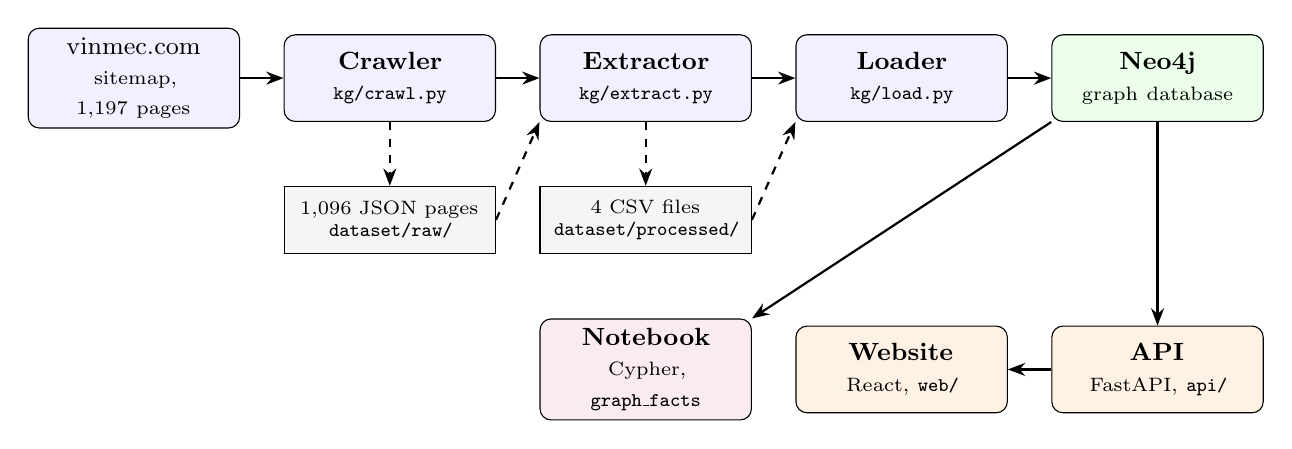
\begin{tikzpicture}[
    box/.style={draw, rounded corners, fill=blue!6, minimum height=1.1cm, text width=2.45cm, align=center, font=\small},
    file/.style={draw, fill=gray!8, minimum height=0.85cm, text width=2.45cm, align=center, font=\scriptsize},
    arr/.style={-{Stealth[length=2.2mm]}, thick}]
\node[box] (web) at (0,0) {vinmec.com\\ \scriptsize sitemap, 1,197 pages};
\node[box] (crawl) at (3.25,0) {\textbf{Crawler}\\ \scriptsize\texttt{kg/crawl.py}};
\node[box] (extract) at (6.5,0) {\textbf{Extractor}\\ \scriptsize\texttt{kg/extract.py}};
\node[box] (load) at (9.75,0) {\textbf{Loader}\\ \scriptsize\texttt{kg/load.py}};
\node[box, fill=green!8] (neo) at (13,0) {\textbf{Neo4j}\\ \scriptsize graph database};
\node[file] (raw) at (3.25,-1.8) {1,096 JSON pages\\ \texttt{dataset/raw/}};
\node[file] (csv) at (6.5,-1.8) {4 CSV files\\ \texttt{dataset/processed/}};
\node[box, fill=purple!8] (nb) at (6.5,-3.7) {\textbf{Notebook}\\ \scriptsize Cypher, \texttt{graph\_facts}};
\node[box, fill=orange!10] (site) at (9.75,-3.7) {\textbf{Website}\\ \scriptsize React, \texttt{web/}};
\node[box, fill=orange!10] (api) at (13,-3.7) {\textbf{API}\\ \scriptsize FastAPI, \texttt{api/}};
\draw[arr] (web) -- (crawl);
\draw[arr] (crawl) -- (extract);
\draw[arr] (extract) -- (load);
\draw[arr] (load) -- (neo);
\draw[arr, dashed] (crawl) -- (raw);
\draw[arr, dashed] (raw.east) -- (extract.south west);
\draw[arr, dashed] (extract) -- (csv);
\draw[arr, dashed] (csv.east) -- (load.south west);
\draw[arr] (neo) -- (api);
\draw[arr] (api) -- (site);
\draw[arr] (neo.south west) -- (nb.north east);
\end{tikzpicture}
\caption{System overview. Solid arrows show data flowing between programs, dashed arrows files written to and read from disk. The notebook, the Cypher queries and the website all read the same Neo4j database.}
\label{fig:overview}
\end{figure}

% =====================================================================
\section{Problem Definition}
\label{sec:problem}

\subsection{Input and Output}

\textbf{Input.} The public Vietnamese diabetes articles of vinmec.com: the official disease pages (short structured summaries with fixed headings for overview, causes, symptoms, risk groups, prevention, diagnosis and treatment) and the much larger set of advice articles written or reviewed by Vinmec doctors. No other source is used.

\textbf{Output.} A Knowledge Graph in which
\begin{itemize}
    \item each node is a named diabetes concept with a type: a form of diabetes, symptom, risk factor, complication, test, drug, drug class, food, lifestyle measure or organ;
    \item each edge is a fact with a named relation such as \code{HAS\_SYMPTOM} or \code{TREATED\_BY};
    \item each extracted fact records how many different articles state it (its \textbf{support}) and which ones;
\end{itemize}
together with three ways to use it: Cypher queries in Neo4j, a retrieval function returning the facts around one entity, and a website.

\subsection{Questions the System Must Answer}

A graph is useful only if it answers real questions. The design started from what a reader of diabetes articles would ask, and each question calls for a different query shape (Table~\ref{tab:questions}).

\begin{table}[H]
\centering
\small
\caption{Questions the system must answer and the query each one needs.}
\label{tab:questions}
\begin{tabularx}{\textwidth}{X l X}
\toprule
Question & Query type & What the graph must hold \\
\midrule
What are the symptoms of type 1 diabetes? Which drugs treat type 2? & one-hop & typed facts from each diabetes type \\
What do we know about Metformin? & one-hop, both directions & facts where Metformin is subject or object \\
Which organs can type 2 diabetes damage? & two-hop & complications \emph{and} the organ each affects \\
Which types of diabetes match these symptoms? & aggregation over one hop & symptom facts per type, with support \\
How is obesity connected to the kidney? & shortest path & a connected graph \\
How is diabetes diagnosed, at which values? & one-hop + node property & tests with thresholds on the test nodes \\
Where does this fact come from? & provenance & article URLs stored on each fact \\
\bottomrule
\end{tabularx}
\end{table}

These questions shaped the design. The two-hop question is why \emph{affects organ} facts were added by hand (Section~\ref{sec:curated}); the symptom checker is why support is kept on every fact instead of being used once as a filter; the provenance question is why articles are nodes in the graph.

\subsection{Success Criteria}

\begin{enumerate}
    \item \textbf{Size and structure} (Mini Project 3, Exercise 1): at least 50 entities, 100 relationships, 5 relation types, 3 entity types; triples in CSV; at least five Cypher queries including one-hop and two-hop; a visualisation.
    \item \textbf{Correctness}, measured and not assumed: a random sample of facts is checked by hand against the source articles, and precision is reported with its uncertainty.
    \item \textbf{Traceability}: every extracted fact links to the articles behind it.
    \item \textbf{Usability}: someone who knows no Cypher can find an entity, see its facts and sources, compare diabetes types, check symptoms and find connections.
\end{enumerate}

\subsection{What the System Is Not}

The graph summarises what public health articles say. It is neither a diagnostic tool nor medical advice. ``Correct'' in this report means that the Vinmec articles state the fact for that form of diabetes, not that a physician verified it against current guidelines. The website and the evaluation both repeat this, since on a medical topic the difference matters.

% =====================================================================
\section{Data Collection}
\label{sec:data}

\subsection{Why Vinmec}

Three properties make Vinmec a good single source for a Vietnamese diabetes graph. The articles are in Vietnamese, so the graph uses the words readers actually use. Coverage is wide: nearly a thousand diabetes articles span early signs, diet, drugs and pregnancy. And the writing is consistent: doctors write or review it, and it follows recognisable headings such as \emph{Triệu chứng} (symptoms), \emph{Nguyên nhân} (causes) and \emph{Điều trị} (treatment). Section~\ref{sec:extraction} shows that this regularity is what makes automatic extraction feasible.

\subsection{Finding the Pages}

\paragraph{Why not the search box.} A program cannot use the site's search: results are drawn by JavaScript in the browser, so downloading the search page yields the page before any results exist. A test request for ``tiểu đường'' returned about 150~KB of HTML with no article links.

\paragraph{The sitemap.} Websites publish a \textbf{sitemap}, a file listing every URL so that search engines can index them. Vinmec's \code{sitemap.xml} points to about 230 smaller sitemaps. The crawler reads those for Vietnamese articles (\code{posts-vi-*}) and Vietnamese disease pages (\code{diseases-vi-*}), which together list around 222,000 URLs: the whole Vietnamese site.

\paragraph{Selecting by slug.} Each URL ends in a readable name called the \textbf{slug}, written without accents; the article \emph{``Bệnh đái tháo đường: chế độ ăn như thế nào?''} has the slug \code{benh-dai-thao-duong-che-do-nhu-nao-vi}. Selecting by slug avoids downloading all 222,000 pages. Keywords come in two strengths because their risks differ:
\begin{itemize}
    \item \textbf{strong} (\code{tieu-duong}, \code{thao-duong}, \code{dai-duong}): a slug containing one is almost certainly about diabetes;
    \item \textbf{weak} (\code{insulin}, \code{metformin}, \code{hba1c}, \code{duong-huyet} = blood sugar, \code{glucose}, \code{sglt2}\ldots): the page \emph{may} be about diabetes, but these words also occur in articles on other subjects, such as the role of insulin in the body or blood sugar in healthy people.
\end{itemize}
The slug \code{thao-nhat} is excluded: \emph{đái tháo nhạt} (diabetes insipidus) shares ``đái tháo'' with \emph{đái tháo đường} but is a different disease of kidneys and hormones.

This yields \textbf{1,197 candidate URLs}. A few either failed to download or duplicated an article under a second address (the crawler skips a title it has already seen), so \textbf{1,191 pages} were downloaded and checked: 944 with a strong keyword and 247 with only a weak one.

\paragraph{Politeness.} The site's \code{robots.txt}, which states what automated programs may fetch, permits these paths. The crawler identifies itself as a student research crawler, waits one second between requests, retries failures with growing pauses, saves each page as soon as it is processed and skips pages already saved, so an interrupted crawl resumes where it stopped.

\subsection{Why a Second Filter Is Needed}

Selecting by slug has a flaw caused by the missing accents. Vietnamese has many words that differ only by accent, and without accents they coincide:
\begin{itemize}
    \item \code{tieu-duong} is \emph{tiểu đường} (diabetes), but also the start of \emph{tiểu dương vật} (a urology question about a child);
    \item \code{dai-duong} is \emph{đái đường}, but also \emph{đại dương} (ocean), as in \emph{cá ngừ đại dương};
    \item \code{duong} also hides \emph{dưỡng ẩm} (moisturising) and \emph{dương tính} (a positive test result).
\end{itemize}
These pages pass the slug test and have nothing to do with diabetes. After downloading, each page is therefore rechecked on its real text, \textbf{with accents}, where such words are distinct. The check counts how often the page mentions diabetes (\emph{tiểu đường}, \emph{đái tháo đường}, \emph{ĐTĐ}: the ``diabetes count'') and how often it uses related terms (\emph{đường huyết}, \emph{insulin}, \emph{HbA1c}, \emph{biến chứng}\ldots: the ``related count''). A page is kept if:

\begin{enumerate}
    \item it is an official Vinmec \textbf{disease page}, already classified by Vinmec; or
    \item its \textbf{title or summary} mentions diabetes and the text does so at least twice (the title is the author's own statement of the topic, the strongest signal); or
    \item its slug had a \textbf{strong} keyword and the text mentions diabetes at least three times, which removes accent collisions (they mention it zero times); or
    \item its slug had only a \textbf{weak} keyword and the text mentions diabetes at least five times \emph{and} uses related terms at least five times. An article ``Insulin là gì?'' that names the hormone thirty times and diabetes once is about biology, not the disease.
\end{enumerate}

The thresholds are loose where evidence is strong (the title) and strict where a wrong page is likely (a weak keyword). Table~\ref{tab:relevance} gives the outcome and Table~\ref{tab:rejected} some rejected pages.

\begin{table}[H]
\centering
\small
\caption{Candidate pages kept and rejected by the relevance filter, by slug keyword strength.}
\label{tab:relevance}
\begin{tabular}{lrrr}
\toprule
Slug keyword & Kept & Rejected & Checked \\
\midrule
\tabinput{table_relevance.tex}
\bottomrule
\end{tabular}
\end{table}

\begin{table}[H]
\centering
\small
\caption{Examples of rejected pages with their diabetes and related counts. The first four are accent collisions.}
\label{tab:rejected}
\begin{tabularx}{\textwidth}{X l r r}
\toprule
Title & Slug keyword & Diabetes count & Related count \\
\midrule
\tabinput{table_rejected.tex}
\bottomrule
\end{tabularx}
\end{table}

Only 10 of 944 strong-keyword pages were rejected, all of them collisions like \emph{tiểu dương vật} and \emph{đại dương}. Of the weak-keyword pages, about a third were rejected as being about insulin, blood sugar or tests in general. The filter is imperfect: a short article on a winter-melon remedy for diabetes falls under the threshold. Losing a few short pages costs little, while admitting off-topic ones would put false facts into the graph.

\subsection{Parsing a Page}

The crawler does not store raw HTML, in which menus, advertisements, booking forms, footers and scripts outweigh the article. It uses the structure of Vinmec's pages:
\begin{itemize}
    \item \textbf{articles}: the body is the element of class \code{entry}; title, date, author and summary come from the structured metadata (\code{application/ld+json}) that search engines read;
    \item \textbf{disease pages}: each section is an element of class \code{item\_detial\_sick} holding a heading and a body.
\end{itemize}
The body is split into \textbf{sections}, and for each the crawler saves the \textbf{heading}, the \textbf{paragraphs} and the \textbf{bullet points} separately.

Keeping the heading is the most consequential design decision in the project. The heading says what kind of information the text below it holds: the bullet ``Mệt mỏi'' (fatigue) means one thing under \emph{Triệu chứng} and another under \emph{Tác dụng phụ của thuốc} (side effects). Section~\ref{sec:extraction} builds on this.

Text at the end of an article that is not part of it is removed: the booking message (\emph{``Để đặt lịch khám tại viện, Quý khách vui lòng bấm số HOTLINE\ldots''}), the app advert and the ``Xem thêm:'' (see also) links. Left in, every article would ``mention'' the same booking phrases and the links would import words from unrelated topics. Figure~\ref{fig:page} shows the saved form of the type 2 disease page.

\begin{figure}[H]
\centering
\begin{codeblock}
title: Tiểu đường tuýp 2: Nguyên nhân, triệu chứng, chẩn đoán và điều trị
url:   https://www.vinmec.com/vie/benh/tieu-duong-tuyp-2-3042     type: disease

## Tổng quan bệnh Tiểu đường tuýp 2            (4 paragraphs, 0 bullets)
## Nguyên nhân bệnh Tiểu đường tuýp 2          (1 paragraph,  0 bullets)
## Triệu chứng bệnh Tiểu đường tuýp 2          (3 paragraphs, 4 bullets)
     • Ăn nhiều
     • Uống nhiều (hay khát nước)
     • Tiểu nhiều (do đường trong nước tiểu cao, gây lợi niệu thẩm thấu)
     • Gầy nhiều (gầy sút cân): bệnh nhân tiểu đường tuýp 2 thường có ...
## Biến chứng cấp tính                         (1 paragraph,  0 bullets)
## Biến chứng mạn tính                         (0 paragraphs, 6 bullets)
     • Nhìn mờ (do biến chứng võng mạc, đục thủy tinh thể)
     • Tê bì dị cảm ở bàn chân (biến chứng thần kinh)
     ...
## Đối tượng nguy cơ bệnh Tiểu đường tuýp 2    ...
## Các biện pháp chẩn đoán bệnh Tiểu đường tuýp 2  ...
## Các biện pháp điều trị bệnh Tiểu đường tuýp 2   ...
\end{codeblock}
\caption{Vinmec's type 2 disease page as saved: sections, each with heading, paragraphs and bullets (abridged).}
\label{fig:page}
\end{figure}

\subsection{Data Volume}

\begin{table}[H]
\centering
\small
\caption{Size of the collected corpus.}
\label{tab:volume}
\begin{tabular}{lr}
\toprule
Quantity & Value \\
\midrule
\tabinput{table_volume.tex}
\bottomrule
\end{tabular}
\end{table}

\begin{figure}[H]
\centering
\includegraphics[width=\textwidth]{corpus_stats.png}
\caption{Left: words per kept page. Middle: diabetes mentions per page (clipped at 60). Right: publication year of kept pages.}
\label{fig:corpus}
\end{figure}

Figure~\ref{fig:corpus} sketches the corpus. A typical page runs to about a thousand words, enough for several aspects of the disease under separate headings. Half of the kept pages mention diabetes 16 times or more and few mention it fewer than six times, which confirms the filter kept pages about the disease and not passing mentions. Nearly all dated pages (1,083 of 1,092) carry a 2024 date. That is when Vinmec republished its archive, not when each article was written, so true article age is unknown; Section~\ref{sec:limitations} returns to this.

% =====================================================================
\section{Knowledge Graph Design}
\label{sec:kg}

\subsection{Facts, Entities and Relations}

A Knowledge Graph is a set of \textbf{triples}, each stating one fact in a fixed three-part form: what the fact is about (the \textbf{subject}), the kind of link (the \textbf{relation}) and the other thing (the \textbf{object}). The part of the type 2 disease page that lists classic symptoms and chronic complications becomes:

\begin{center}
\small
\begin{tabular}{lll}
\toprule
subject & relation & object \\
\midrule
Đái tháo đường type 2 & HAS\_SYMPTOM & Khát nhiều \\
Đái tháo đường type 2 & HAS\_SYMPTOM & Tiểu nhiều \\
Đái tháo đường type 2 & HAS\_COMPLICATION & Bệnh võng mạc \\
Bệnh võng mạc & AFFECTS\_ORGAN & Mắt \\
\bottomrule
\end{tabular}
\end{center}

This beats the paragraph because every fact has the same predictable form. A program need not parse Vietnamese grammar; it looks for facts whose subject is ``type 2'' and relation \code{HAS\_COMPLICATION}. The ambiguity of language is settled once, when the fact is made, not at every question.

Draw each thing as a dot and each fact as an arrow and the facts become a \textbf{graph}: the things are \textbf{nodes} or \textbf{entities}, the facts \textbf{edges} or \textbf{relationships}, and each node has a \textbf{type} (\code{Symptom}, \code{Drug}\ldots). Figure~\ref{fig:toy} draws seven hand-written facts. Questions become walks: ``which organ does type 2 damage?'' goes from \emph{type 2} along \code{HAS\_COMPLICATION} to \emph{Bệnh thận đái tháo đường}, then along \code{AFFECTS\_ORGAN} to \emph{Thận}. No single fact holds the answer; two facts joined at the middle node do. The lecture calls this a \textbf{two-hop} query, as opposed to a \textbf{one-hop} query that reads only the arrows touching one node.

\begin{figure}[H]
\centering
\includegraphics[width=0.72\textwidth]{toy_graph.png}
\caption{Seven hand-written diabetes facts as a graph (notebook, Part 1). The kidney (\emph{Thận}) is two hops from \emph{type 2}: no single fact joins them.}
\label{fig:toy}
\end{figure}

The real graph has the same shape but is built automatically from 1,096 articles. The hard part of the project is not storing the graph but extracting \textbf{correct} facts from free Vietnamese text without anyone reading every article, and the rest of this section explains how.

\subsection{Schema: Entity Types and Relation Types}
\label{sec:schema}

The schema says which kinds of entities exist and which facts may link them. It was designed from the questions of Table~\ref{tab:questions} and from the layout of Vinmec's articles.

\textbf{Entity types.} There are ten (Table~\ref{tab:entity-types}). Five mirror the standard sections of a disease article: symptoms, risk factors, complications, tests and treatments. Treatments split into \code{Drug} and \code{Lifestyle} since the questions differ (``which drug class?'' makes sense only for drugs). \code{Food} is separate because diet is among the most discussed topics. \code{DrugClass} and \code{Organ} are not extracted from text: they group drugs and place complications in the body (Section~\ref{sec:curated}). The five \code{DiabetesType} nodes are the subjects of almost every extracted fact.

\begin{table}[H]
\centering
\small
\caption{Entity types: vocabulary entries, aliases (spellings), entities that reached the graph, and the best-connected examples.}
\label{tab:entity-types}
\begin{tabularx}{\textwidth}{l r r r X}
\toprule
Type & Vocabulary & Aliases & In graph & Examples \\
\midrule
\tabinput{table_entity_types.tex}
\bottomrule
\end{tabularx}
\end{table}

Nearly every vocabulary entry earned enough support to enter the graph; the one complication and one risk factor that did not are discussed in Section~\ref{sec:errors}.

\textbf{Relation types.} Table~\ref{tab:relations} lists the twelve relations with the entity types they join and their fact counts. The \code{source} column separates facts extracted from articles (\code{vinmec}) from general classifications added by hand (\code{curated}).

\begin{table}[H]
\centering
\small
\caption{Relation types in the graph.}
\label{tab:relations}
\begin{tabular}{l l l r}
\toprule
Relation & From $\rightarrow$ to & Source & Facts \\
\midrule
\tabinput{table_relations.tex}
\bottomrule
\end{tabular}
\end{table}

The direction of each relation is a modelling choice: \code{HAS\_SYMPTOM} runs from disease to symptom but could be \code{SYMPTOM\_OF} the other way. The convention here is that facts point \emph{away} from the diabetes types and on to classifications. Section~\ref{sec:pagerank} shows this choice matters for graph measures. Figure~\ref{fig:schema} draws the schema: each arrow is a question the graph can answer, and a missing arrow (say \code{Food} to \code{Complication}) is a question it cannot.

\begin{figure}[H]
\centering
\includegraphics[width=0.92\textwidth]{schema.png}
\caption{The schema as stored in Neo4j: entity types (circles) and the relations between them with fact counts. Diabetes types on the left, what the articles say about them in the middle, hand-added classifications on the right.}
\label{fig:schema}
\end{figure}

\subsection{Extraction Method}
\label{sec:extraction}

\subsubsection{Why a bullet point should not become a node}

The simplest scheme would make every bullet under \emph{Triệu chứng} a Symptom node. On the type 2 page that gives acceptable nodes such as ``Ăn nhiều''. But a bullet under \emph{Điều trị} on the type 1 page reads:

\begin{quote}\small
\emph{``Kiểm soát đường huyết: đối với tuýp 1 thì kiểm soát bằng insulin ngoại sinh là chủ yếu. Dùng theo phác đồ, tuân thủ giờ tiêm và liều lượng tránh bị tụt đường huyết. Các loại insulin gồm có\ldots''}
\end{quote}

Sixty words make a useless node: no other article repeats them, so it links to nothing and matches no question. Even short bullets differ between articles (\emph{uống nhiều}, \emph{khát nước}, \emph{hay khát}), so a single fact ``diabetes causes thirst'' would shatter into weak pieces that never meet.

The project therefore decides \textbf{in advance} which concepts the graph may contain, names each cleanly, and searches the text for every way of writing it. For every section of every page, extraction then answers three questions:
\begin{enumerate}
    \item \textbf{Which diabetes is the page about?} That is the subject.
    \item \textbf{What may this section contain?} The heading decides.
    \item \textbf{Which known concepts does it mention?} Those are the objects.
\end{enumerate}
Each fact found on a page is one \textbf{vote} from that page; votes are tallied, and a fact enters the graph only when enough different pages agree. Figure~\ref{fig:pipeline} traces a real section.

\begin{figure}[H]
\centering
\begin{tikzpicture}[
    st/.style={draw, rounded corners, fill=blue!5, text width=3.05cm, align=left, font=\scriptsize, minimum height=2.5cm},
    lab/.style={font=\small\bfseries, align=center},
    arr/.style={-{Stealth[length=2mm]}, thick},
    node distance=0.35cm]
\node[st] (a) {\textbf{Page title}\\ ``Tiểu đường tuýp 2: Nguyên nhân, triệu chứng\ldots''\\[3pt] $\Rightarrow$ subject:\\ \textbf{Đái tháo đường type 2}};
\node[st, right=of a] (b) {\textbf{Section heading}\\ ``Triệu chứng bệnh Tiểu đường tuýp 2''\\[3pt] contains \emph{triệu chứng}, names the disease\\ $\Rightarrow$ allowed: \textbf{Symptom}};
\node[st, right=of b] (c) {\textbf{Bullets}\\ ``Ăn nhiều'', ``Uống nhiều (hay khát nước)'', ``Tiểu nhiều \ldots'', ``Gầy nhiều (gầy sút cân)''\\[3pt] aliases matched $\Rightarrow$ Ăn nhiều, Khát nhiều, Tiểu nhiều, Sụt cân};
\node[st, right=of c] (d) {\textbf{This page's votes}\\ (type 2, HAS\_SYMPTOM, Khát nhiều) \ldots\\[3pt] tallied over all 1,096 pages; kept if $\geq$ 2 pages (or a disease page)};
\draw[arr] (a) -- (b); \draw[arr] (b) -- (c); \draw[arr] (c) -- (d);
\node[lab, above=0.15cm of a] {1. subject};
\node[lab, above=0.15cm of b] {2. allowed types};
\node[lab, above=0.15cm of c] {3. objects};
\node[lab, above=0.15cm of d] {4. support};
\end{tikzpicture}
\caption{Extracting symptom facts from the symptom section of Vinmec's type 2 disease page.}
\label{fig:pipeline}
\end{figure}

\subsubsection{The vocabulary and entity normalisation}

The vocabulary (\code{kg/vocab.py}) lists 106 concepts, each with a clean \textbf{canonical name} that becomes the node, a \textbf{type}, and \textbf{aliases}, the spellings found in articles (320 in all). A sample:

\begin{codeblock}
VOCAB = {
    "Khát nhiều":    ("Symptom", ["khát nhiều", "uống nhiều", "khát nước", "hay khát", "khô miệng"]),
    "Tê bì tay chân": ("Symptom", ["tê bì", "tê tay", "tê chân", "dị cảm", "ngứa ran", "kiến bò"]),
    "Kháng insulin": ("RiskFactor", ["kháng insulin", "đề kháng insulin"]),
    "Bệnh võng mạc": ("Complication", ["võng mạc", "biến chứng mắt", "mù lòa"]),
    "HbA1c":         ("Test", ["hba1c", "hemoglobin a1c", "a1c"]),
    "Metformin":     ("Drug", ["metformin", "glucophage"]),
    "Empagliflozin": ("Drug", ["empagliflozin", "jardiance"]),
    "Rau xanh":      ("Food", ["rau xanh", "rau lá xanh", "rau củ", "bông cải", "súp lơ"]),
    ...
}
\end{codeblock}

Mapping many spellings to one node is \textbf{entity normalisation}, and it is what lets evidence accumulate: an article saying \emph{uống nhiều} and another saying \emph{khát nước} both vote for \emph{(diabetes, HAS\_SYMPTOM, Khát nhiều)}. Brand names (\emph{Glucophage}, \emph{Diamicron}, \emph{Januvia}, \emph{Jardiance}, \emph{Lantus}) are aliases because Vietnamese articles often name drugs by brand.

The list was written by hand from the topics the articles cover: classic symptoms, risk factors on Vinmec's pages, acute and chronic complications, standard tests, drugs used in Vietnam, and the foods and lifestyle measures of diet articles. The price is plain, a concept missing from the list can never be found, and so is the benefit, every node is clean, meaningful and correctly typed. Section~\ref{sec:limitations} weighs the price.

\subsubsection{Matching aliases in text}

All aliases of an entity are compiled into one regular expression. For \emph{Tiểu nhiều}:
\begin{codeblock}
(?<!\w)(đi tiểu thường xuyên|tiểu thường xuyên|đi tiểu nhiều|tiểu nhiều|tiểu đêm)(?!\w)
\end{codeblock}
Three details matter.

\textbf{Whole words only.} Vietnamese separates syllables with spaces, and many aliases are one short syllable that also occurs inside longer words: the fruit \emph{lê} (pear) would match inside \emph{lên} (as in \emph{lên cân}, gaining weight) and \emph{bia} (beer) inside \emph{biên}. The lookarounds \code{(?<!\textbackslash w)} and \code{(?!\textbackslash w)} demand non-letters on both sides, so ``bệnh nhân lên cân'' contains no food while ``ăn quả lê'' does.

\textbf{Longest alias first.} Were ``tiểu thường xuyên'' tried before ``đi tiểu thường xuyên'', the short form would win and the more specific wording never be used.

\textbf{Accents stay.} Text is lower-cased so ``HbA1C'' equals ``hba1c'', but accents are never stripped, which would revive the URL problem (\emph{tiểu đường} equals \emph{tiểu dương}).

Word boundaries cannot stop an alias that is a whole word with a second meaning: the fruit \emph{táo} (apple) matches \emph{táo bón} (constipation). The section rule below keeps such errors rare, because a food alias counts only inside diet sections.

\subsubsection{The section rule: the heading decides}
\label{sec:section-rule}

Finding a vocabulary word in an article does not mean the article asserts something about it. Real cases from the corpus:
\begin{itemize}
    \item \emph{mệt mỏi} appears in a diet article (``ăn sáng đầy đủ giúp bạn đỡ mệt mỏi''), which does not say fatigue is a symptom of diabetes;
    \item \emph{tăng huyết áp} appears in drug paragraphs as a condition the drug should not be combined with;
    \item nearly every article says \emph{insulin} while explaining blood sugar, not because insulin is the treatment under discussion.
\end{itemize}
If every match counted, diabetes would acquire dozens of ``symptoms'' that are just words that happened to occur. A match therefore counts only when the \textbf{section heading} says the section is about that kind of information, which works because hospital articles are organised under exactly such headings (Table~\ref{tab:section-rule}).

\begin{table}[H]
\centering
\small
\caption{The section rule: heading keywords and the entity types extractable below them.}
\label{tab:section-rule}
\begin{tabularx}{\textwidth}{X l l}
\toprule
Heading contains & Allowed types & Relation produced \\
\midrule
triệu chứng, dấu hiệu, biểu hiện, nhận biết & Symptom & HAS\_SYMPTOM \\
nguyên nhân, nguy cơ, đối tượng, yếu tố, ai dễ & RiskFactor & HAS\_RISK\_FACTOR \\
biến chứng, nguy hiểm, hậu quả, ảnh hưởng & Complication & HAS\_COMPLICATION \\
chẩn đoán, xét nghiệm, phát hiện, chỉ số, kiểm tra, theo dõi & Test & DIAGNOSED\_BY \\
điều trị, thuốc, insulin, kiểm soát & Drug, Lifestyle & TREATED\_BY, MANAGED\_BY \\
phòng ngừa, phòng tránh, ngăn ngừa, lối sống, lưu ý & Lifestyle & MANAGED\_BY \\
ăn, thực phẩm, dinh dưỡng, thực đơn, món, uống, kiêng, tránh & Food & RECOMMENDS\_FOOD / AVOIDS\_FOOD \\
\bottomrule
\end{tabularx}
\end{table}

A section whose heading has none of these keywords, such as \emph{Tổng quan} (overview), yields no facts. This is intended: an overview mentions everything in passing, and missing a fact is preferable to inventing one.

\paragraph{A second check for symptoms and risk factors.} The quality audit in Section~\ref{sec:precision} exposed a gap in the first version. A heading may contain \emph{nguyên nhân} or \emph{nguy cơ} without being about diabetes:
\begin{itemize}
    \item \emph{``Một số nguyên nhân gây ngứa bàn tay và bàn chân''} lists causes of \textbf{itching};
    \item \emph{``Yếu tố nguy cơ gây tai biến mạch máu não ở người tiểu đường''} lists risks of \textbf{stroke} in people who already have diabetes;
    \item \emph{``Làm gì để giảm thiểu nguy cơ tim mạch\ldots''} gives advice on \textbf{lowering} a risk.
\end{itemize}
Reading these bullets as risk factors \emph{of diabetes} produced false facts. A symptom or risk factor always belongs to \emph{something}, and the heading names it. For these two types only, the heading must therefore also pass \code{about\_disease()}:

\begin{codeblock}
DISEASE_TERMS = ["tiểu đường", "đái tháo đường", "đtđ", "tuýp", "type", "típ", "bệnh"]
OTHER_TOPIC   = ["biến chứng", "thận", "võng mạc", "mắt", "thần kinh", "bàn chân", "tim mạch",
                 "ngứa", "gout", "da", "răng", "nhiễm toan", "ceton", "hạ đường huyết",
                 "thai nhi", "trẻ sinh ra", "tai biến", "đột quỵ", "mạch vành", "hôn mê"]
REDUCE_VERBS  = ["giảm", "phòng", "tránh", "ngừa", "hạn chế", "kiểm soát"]

def about_disease(heading):
    """Generic heading ("Triệu chứng", "Ai dễ bị?") or one that names diabetes, and no other topic."""
    h = re.sub(r"^[\d\.\s]+", "", heading.lower())          # drop numbering such as "2.1."
    if any(t in h for t in OTHER_TOPIC) or any(v + " nguy cơ" in h for v in REDUCE_VERBS):
        return False
    return any(t in h for t in DISEASE_TERMS) or len(h.split()) <= 5

def allowed_labels(heading):
    h = heading.lower()
    labels = set()
    for keys, labs in SECTION_RULES:                          # the rule of Table 7
        if any(k in h for k in keys):
            labels |= labs
    if not about_disease(heading):
        labels -= {"Symptom", "RiskFactor"}
    return labels
\end{codeblock}

So the heading must name diabetes or be short and generic (``Triệu chứng'', ``Ai dễ bị?'', which can only refer to the disease), must name no other topic, and must not be about reducing a risk. Table~\ref{tab:headings} applies the rule to real headings.

\begin{table}[H]
\centering
\small
\caption{The section rule applied to real headings.}
\label{tab:headings}
\begin{tabularx}{\textwidth}{X c l}
\toprule
Heading & About diabetes itself? & Allowed types \\
\midrule
Triệu chứng bệnh Tiểu đường tuýp 2 & yes & Symptom \\
Đối tượng nguy cơ bệnh Tiểu đường tuýp 1 & yes & RiskFactor \\
3. Ai dễ bị tiền tiểu đường? & yes & RiskFactor \\
Các biện pháp điều trị bệnh Tiểu đường tuýp 1 & yes & Drug, Lifestyle \\
2.2. Một số thực phẩm mẹ bầu mắc bệnh tiểu đường thai kỳ cần tránh & yes & Food \\
3. Một số nguyên nhân gây ngứa bàn tay và bàn chân & no & -- \\
2. Yếu tố nguy cơ gây tai biến mạch máu não ở người tiểu đường & no & -- \\
4. Làm gì để giảm thiểu nguy cơ tim mạch ở bệnh nhân tiểu đường? & no & -- \\
Biến chứng mạn tính & yes & Complication \\
\bottomrule
\end{tabularx}
\end{table}

\subsubsection{Which diabetes is the subject?}

Diabetes is several diseases. Type 1 is autoimmune loss of insulin-producing cells, usually beginning young. Type 2 develops slowly in adults with weight and lifestyle. Gestational diabetes arises in pregnancy. Prediabetes precedes type 2. Their symptoms, causes and treatments overlap but differ: ``autoimmune destruction of beta cells'' is a type 1 cause only, ``pre-eclampsia'' a gestational complication only. One shared ``diabetes'' node would erase these differences.

Each page therefore gets its subject from the \textbf{title}, the author's own short statement of the topic and more reliable than counting words in the body (a type 2 article often mentions type 1 for comparison). The title is tested in turn for \emph{tuýp 1 / type 1 / típ 1}, \emph{tuýp 2 / type 2}, \emph{thai kỳ / mang thai / mẹ bầu} and \emph{tiền đái tháo đường / tiền tiểu đường}; if none is found, the subject is diabetes in general.

This simplification has a visible effect (Figure~\ref{fig:subjects}): most titles name no type, so the general node collects most facts even though many of those articles concern type 2. It is accepted on purpose, because a type 2 fact on the general node is merely less specific, whereas on the type 1 node it would be false.

\begin{figure}[H]
\centering
\includegraphics[width=0.6\textwidth]{pages_per_subject.png}
\caption{Pages assigned to each subject. Most titles name no specific type.}
\label{fig:subjects}
\end{figure}

\subsubsection{Counting evidence: why one page is not enough}

Every rule above can still fail on one page: an odd heading, a passing mention, a list written for comparison. Trusting each page would turn each slip into a fact. The defence is \textbf{agreement between independent pages}. For every fact the extractor keeps the \emph{set} of pages that voted for it (a set, so a page repeating ``khát nhiều'' five times counts once), and the size of that set is the fact's \textbf{support}.

Example, with three pages about type 2:

\begin{center}
\small
\begin{tabular}{ll}
\toprule
Page & Facts it votes for \\
\midrule
A & type 2 HAS\_SYMPTOM Khát nhiều; type 2 HAS\_SYMPTOM Mệt mỏi \\
B & type 2 HAS\_SYMPTOM Khát nhiều \\
C & type 2 HAS\_SYMPTOM Khát nhiều; type 2 HAS\_SYMPTOM Run tay \\
\bottomrule
\end{tabular}
\end{center}

\emph{Khát nhiều} has support 3 and is kept; \emph{Mệt mỏi} and \emph{Run tay} have support 1 and are dropped, the same logic as checking a claim against a second source. There are two exceptions, each with a reason:
\begin{itemize}
    \item a fact from an official Vinmec \textbf{disease page} is accepted at support 1, since these are short, hospital-reviewed summaries with exactly the standard headings and so the most reliable input;
    \item a \textbf{side effect} needs support 3, because it is read from single sentences and is noisier (below).
\end{itemize}

\begin{codeblock}
for (h, rel, t), urls in support.items():                 # urls = set of pages voting for the fact
    need = MIN_SUPPORT_SIDE_EFFECT if rel == "HAS_SIDE_EFFECT" else MIN_SUPPORT   # 3 or 2
    if len(urls) >= need or (h, rel, t) in from_disease:
        triples.append((h, rel, t, len(urls), "vinmec", " ".join(sorted(urls)[:5])))
\end{codeblock}

The support number survives the filter and is stored on the fact in Neo4j, so queries can rank by documentation, and the website lets the reader hide facts below a chosen level.

\subsubsection{Foods: recommended or avoided}

The graph distinguishes \code{RECOMMENDS\_FOOD} from \code{AVOIDS\_FOOD}. The first attempt decided from cue words in the sentence or heading (\emph{nên ăn} for recommended; \emph{kiêng}, \emph{tránh}, \emph{hạn chế}, \emph{không nên} for avoid) and failed, instructively: diet articles mix both kinds of advice together. The heading \emph{``Thực phẩm mẹ bầu cần tránh và nên ăn''} has both cues, and one sentence may say ``hạn chế đồ ngọt, thay vào đó nên ăn rau xanh''. The output included absurdities like \emph{gestational diabetes AVOIDS green vegetables}.

The final rule makes good-or-bad a \textbf{property of the food}, recorded once in the vocabulary: sweets, soft drinks, white rice and refined starch, very sweet fruit (durian, ripe mango, longan, jackfruit), alcohol, fried food and processed meat are ``avoid'', the rest ``recommended''. The text then only shows that the food is discussed in a diet section for that type. This matches standard nutrition advice in nearly all cases; it cannot express nuance such as ``fruit is fine in moderation''.

\subsubsection{Drug side effects}

Side effects are scattered across drug sections, complication sections and general articles, so the section rule cannot find them. They are read \textbf{within one sentence}: the sentence must contain a drug, a symptom or complication, and a causal cue, \emph{tác dụng phụ} (side effect), \emph{tác dụng không mong muốn} or \emph{gây} (causes):

\begin{quote}\small
``Insulin có thể \textbf{gây hạ đường huyết} nếu tiêm quá liều'' $\Rightarrow$ (Insulin, HAS\_SIDE\_EFFECT, Hạ đường huyết)
\end{quote}

Sentences containing \emph{thiếu} (lack of) or \emph{không đủ} are skipped. ``\emph{thiếu} insulin gây nhiễm toan ceton'' has a drug, a complication and \emph{gây}, yet says that a \emph{lack} of insulin causes ketoacidosis, the reverse of a side effect. Without the exception the graph would accuse insulin of causing the condition it treats. Section~\ref{sec:errors} shows the filter catches most but not all such sentences.

\subsubsection{Background facts added by hand}
\label{sec:curated}

Some knowledge is not stated under any heading but is general medical classification that articles assume: Metformin is a biguanide, diabetic retinopathy affects the eye, the diagnostic threshold of HbA1c is 6.5\%. These are added by hand and labelled \code{source = curated}, so they can always be separated from extracted facts:
\begin{itemize}
    \item each drug and its \textbf{class} (22 facts, e.g.\ Metformin $\rightarrow$ Biguanide, Empagliflozin $\rightarrow$ Ức chế SGLT2);
    \item each complication and the \textbf{organ} it affects (12 facts);
    \item each form of diabetes as a \textbf{subtype} of diabetes in general (4 facts);
    \item diagnostic \textbf{thresholds} stored on four test nodes, from the Vietnamese Ministry of Health 2020 guideline and the American Diabetes Association criteria that Vinmec also quotes: HbA1c $\geq$ 6.5\%; fasting plasma glucose $\geq$ 7.0~mmol/L; 2-hour glucose in the tolerance test $\geq$ 11.1~mmol/L; random glucose $\geq$ 11.1~mmol/L with symptoms.
\end{itemize}
These few facts enable the most interesting questions. Without ``retinopathy affects the eye'' the graph can say type 2 causes retinopathy but cannot say which organs type 2 damages.

\subsection{Output Files}
\label{sec:outputs}

The extractor writes four CSV files:

\begin{table}[H]
\centering
\small
\caption{Files produced by the extractor (\code{dataset/processed/}).}
\begin{tabularx}{\textwidth}{l X X}
\toprule
File & One row is & Purpose \\
\midrule
\code{entities.csv} & an entity: name, type, threshold & becomes the nodes \\
\code{triples.csv} & a fact: subject, relation, object, support, source, up to five example URLs & becomes the relationships \\
\code{articles.csv} & a crawled page: URL, title, page type, date, subject & traces facts back to articles \\
\code{mentions.csv} & a (page, entity) pair for every entity mentioned anywhere on the page & a looser signal of what each article discusses \\
\bottomrule
\end{tabularx}
\end{table}

The facts file uses the lecture Exercise 1 form \code{subject, relation, object} with three extra columns:

\begin{codeblock}
subject,relation,object,support,source,example_urls
Đái tháo đường type 2,HAS_SYMPTOM,Khát nhiều,4,vinmec,https://www.vinmec.com/vie/bai-viet/...
Đái tháo đường type 2,TREATED_BY,Metformin,11,vinmec,https://www.vinmec.com/vie/bai-viet/...
Metformin,BELONGS_TO_CLASS,Biguanide,0,curated,
Bệnh võng mạc,AFFECTS_ORGAN,Mắt,0,curated,
\end{codeblock}

Table~\ref{tab:example-triples} shows the best-supported extracted fact of each extracted relation.

\begin{table}[H]
\centering
\small
\caption{The best-supported extracted fact of each relation type.}
\label{tab:example-triples}
\begin{tabular}{l l l r}
\toprule
Subject & Relation & Object & Support \\
\midrule
\tabinput{table_example_triples.tex}
\bottomrule
\end{tabular}
\end{table}

\subsection{Meeting the Lecture's Requirements}
\label{sec:checklist}

\begin{table}[H]
\centering
\small
\caption{Lecture requirements (Mini Project 3, Exercise 1) and what the graph achieves.}
\label{tab:checklist}
\begin{tabularx}{\textwidth}{l X X}
\toprule
Requirement & Lecture minimum & This project \\
\midrule
\tabinput{table_checklist.tex}
\bottomrule
\end{tabularx}
\end{table}

% =====================================================================
\section{System Implementation}
\label{sec:implementation}

\subsection{Project Structure}

The system is written in Python (crawler, extractor, loader, API, notebook) and JavaScript (website). Table~\ref{tab:files} lists each part. Every stage reads files or the database and can be rerun alone.

\begin{table}[H]
\centering
\small
\caption{Project structure of \code{graph\_01/}.}
\label{tab:files}
\begin{tabularx}{\textwidth}{l X}
\toprule
Path & Role \\
\midrule
\code{kg/crawl.py} & sitemap $\rightarrow$ candidate URLs $\rightarrow$ download $\rightarrow$ relevance filter $\rightarrow$ \code{dataset/raw/pages/*.json} and \code{index.csv}; resumable \\
\code{kg/vocab.py} & vocabulary (106 entities, 320 aliases), section rules, food polarity, curated classes, organs, thresholds \\
\code{kg/extract.py} & pages $\rightarrow$ votes $\rightarrow$ support filter $\rightarrow$ \code{dataset/processed/*.csv} \\
\code{kg/load.py} & CSV files $\rightarrow$ Neo4j (wipes and reloads; idempotent) \\
\code{kg/retriever.py} & \code{graph\_facts(entity, hops)}: bounded graph retrieval \\
\code{kg/visualize.py} & NetworkX drawings \\
\code{kg/evaluate.py} & draws the random sample for the quality check \\
\code{kg/queries.cypher} & the 15 example queries for Neo4j Browser \\
\code{notebook/01\_diabetes\_kg.ipynb} & explains and runs every stage, with all figures \\
\code{api/} & FastAPI service: read-only Cypher behind a small REST interface \\
\code{web/} & React website for exploring the graph \\
\code{evaluation/manual\_audit.csv} & the 50 sampled facts with the manual judgement \\
\code{report/} & this report and its plan \\
\bottomrule
\end{tabularx}
\end{table}

\subsection{Storing the Graph in Neo4j}
\label{sec:neo4j}

\subsubsection{Why a graph database}

A NetworkX graph, as in the lecture's first examples, lives in a Python process's memory: it disappears when the program ends and every program must rebuild it. A real system needs permanent storage shared by the notebook, the website and ad hoc Cypher queries, with quick answers.

Triples could go into a relational table with three columns, but graph questions are about \emph{paths}, and in SQL each step of a path is another self-join: queries grow long and slow as the table grows. A \textbf{graph database} keeps direct references from each node to its neighbours, so following an arrow is a jump and not a search. \textbf{Neo4j} is the most widely used, and its language \textbf{Cypher} writes a path as ASCII art that resembles the drawing. Neo4j 5 runs locally in a Docker container with its data in the project folder.

\subsubsection{Data model}

\begin{codeblock}
(:Entity:Symptom {name})                       every entity: label Entity + its own type
(:Entity:Test {name, threshold})
(:DiabetesType)-[:HAS_SYMPTOM {support, source, example_urls}]->(:Symptom)
(:Article {url, title, page_type, date})-[:ABOUT]->(:DiabetesType)
(:Article)-[:MENTIONS]->(:Entity)
\end{codeblock}

Three decisions deserve explanation.

\textbf{Two labels per entity.} The type label (\code{Symptom}) allows asking for ``all symptoms''. The shared \code{Entity} label carries one rule for all, that names are unique, so there is never a second ``Metformin'' node, and permits ``everything connected to Metformin'' without knowing neighbour types.

\textbf{Evidence on the relationships.} \code{support}, \code{source} and \code{example\_urls} are relationship properties, so one query returns the answer, its documentation and its articles. Stored elsewhere, each answer would need a second lookup.

\textbf{Articles are nodes too.} Each of the 1,096 articles is an \code{Article} node linked by \code{ABOUT} to its diabetes type and by \code{MENTIONS} to every entity it mentions anywhere (10,083 links). That preserves the path from clean facts back to the original text and answers ``where does this come from?''. Since article nodes and \code{MENTIONS} links are not facts about diabetes, queries about the knowledge restrict themselves to \code{Entity} nodes.

\subsubsection{Loading}

\begin{codeblock}
CREATE CONSTRAINT entity_name IF NOT EXISTS FOR (e:Entity) REQUIRE e.name IS UNIQUE;

UNWIND $rows AS r
MERGE (e:Entity {name: r.name}) SET e:Symptom;          -- one query per entity type

UNWIND $rows AS r
MATCH (h:Entity {name: r.subject}), (t:Entity {name: r.object})
MERGE (h)-[x:HAS_SYMPTOM]->(t)                           -- one query per relation type
SET x.support = r.support, x.source = r.source, x.example_urls = r.example_urls;
\end{codeblock}

\begin{itemize}
    \item \textbf{\code{MERGE}, not \code{CREATE}.} \code{CREATE} always adds, even if an identical node exists; \code{MERGE} looks first and creates only if missing. The loader can run repeatedly without duplicating anything.
    \item \textbf{\code{UNWIND} sends a batch.} Each request has a fixed cost: the 10,083 mention links one by one would be 10,083 round trips, whereas \code{UNWIND} ships one list and lets the database loop. The graph loads in seconds.
    \item \textbf{The uniqueness constraint is an index} on \code{name}, so every query that begins at ``the node called Metformin'' jumps straight to it.
    \item \textbf{Relation types are in the query text.} Cypher cannot take a relationship type or label as a parameter, so the loader groups facts by relation and builds one query per type from the fixed list of twelve.
\end{itemize}

After loading, the database holds 1,223 nodes (127 entities and 1,096 articles) and 11,518 relationships (339 facts, 10,083 mentions and 1,096 \code{ABOUT} links).

\subsection{Querying with Cypher}

A Cypher query describes the \emph{shape} of a path: round brackets for nodes, square brackets inside an arrow for relationships.

\begin{codeblock}
MATCH (t:DiabetesType {name: 'Đái tháo đường type 2'})-[r:HAS_SYMPTOM]->(s:Symptom)
RETURN s.name, r.support
\end{codeblock}

Read left to right: find a \code{DiabetesType} called ``type 2'', follow outgoing \code{HAS\_SYMPTOM} arrows to \code{Symptom} nodes, return each name and the arrow's support. Neo4j uses the name index to land on the type 2 node and then examines only that node's arrows, never scanning the rest. Work grows with the number of arrows followed, not with database size. The fifteen queries of \code{kg/queries.cypher} are presented in Section~\ref{sec:queries}.

\subsection{Graph Retrieval}
\label{sec:retrieval}

In a complete question-answering system (the lecture's Knowledge Graph + RAG design) the graph's role is to give a language model a small set of relevant, reliable facts. \code{kg/retriever.py} implements the lecture's \code{graph\_facts} on Neo4j:

\begin{codeblock}
ONE_HOP = """
MATCH (e:Entity {name: $name})-[r]-(n:Entity)
RETURN startNode(r).name AS s, type(r) AS rel, endNode(r).name AS o, r.support AS support
ORDER BY support DESC"""
TWO_HOP = """
MATCH (e:Entity {name: $name})-[r1]-(m:Entity)-[r2]-(n:Entity) WHERE n <> e
RETURN startNode(r2).name AS s, type(r2) AS rel, endNode(r2).name AS o, r2.support AS support
ORDER BY support DESC"""

def graph_facts(driver, entity, hops=1, limit=30):
    facts, seen = [], set()
    with driver.session() as s:
        for q in [ONE_HOP] + ([TWO_HOP] if hops >= 2 else []):
            for r in s.run(q, name=entity):
                key = (r["s"], r["rel"], r["o"])
                if key not in seen:
                    seen.add(key)
                    facts.append(f"{r['s']} {r['rel']} {r['o']}.")
    return facts[:limit]
\end{codeblock}

It starts at the entity named in the question, gathers facts within one or two steps, writes each as a short sentence, ranks by support and returns at most 30.

\begin{codeblock}
$ python kg/retriever.py "Hạ đường huyết"
Đái tháo đường HAS_COMPLICATION Hạ đường huyết.
Insulin HAS_SIDE_EFFECT Hạ đường huyết.
Đái tháo đường thai kỳ HAS_COMPLICATION Hạ đường huyết.
Metformin HAS_SIDE_EFFECT Hạ đường huyết.
Đái tháo đường type 2 HAS_COMPLICATION Hạ đường huyết.
\end{codeblock}

The bound on hops and facts matters because within a few steps almost everything connects to everything, especially through hubs. One step from \emph{Hạ đường huyết} (hypoglycaemia) yields the 5 precise facts above; two steps yield \textbf{230}, since one neighbour is the general diabetes node, itself linked to most of the graph. Feeding 230 facts to a language model for a question about hypoglycaemia would bury the relevant ones. The lecture calls this ``graph retrieval too broad'' (§23.4), and the remedy used here is its recommendation: start at the entity in the question, stay within one or two hops, rank and truncate.

\subsection{The Website}
\label{sec:website}

\subsubsection{Architecture}

Cypher is powerful but not for the typical reader, so a website makes the graph usable by anyone. It has two parts:
\begin{itemize}
    \item an \textbf{API} (\code{api/}, Python, FastAPI) that accepts simple HTTP requests, runs fixed Cypher against Neo4j and returns JSON;
    \item a \textbf{web client} (\code{web/}, React 18 with Vite and hand-written CSS, the stack of the course's earlier web applications) shown in the browser.
\end{itemize}

\begin{center}
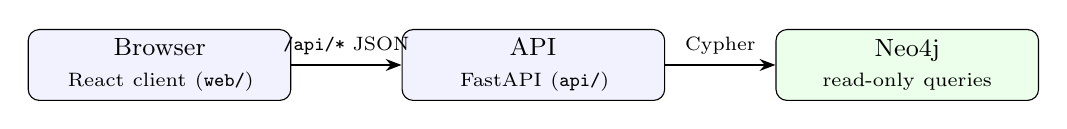
\begin{tikzpicture}[box/.style={draw, rounded corners, fill=blue!5, minimum height=0.9cm, text width=3.1cm, align=center, font=\small}, arr/.style={-{Stealth[length=2mm]}, thick}, node distance=1.4cm]
\node[box] (b) {Browser\\ \scriptsize React client (\code{web/})};
\node[box, right=of b] (a) {API\\ \scriptsize FastAPI (\code{api/})};
\node[box, right=of a, fill=green!8] (n) {Neo4j\\ \scriptsize read-only queries};
\draw[arr] (b) -- node[above, font=\scriptsize]{\code{/api/*} JSON} (a);
\draw[arr] (a) -- node[above, font=\scriptsize]{Cypher} (n);
\end{tikzpicture}
\end{center}

\textbf{Why an API in the middle}, instead of the browser talking to Neo4j directly? Security: the database password stays on the server and the browser can run only the fixed read-only queries the API offers, never arbitrary Cypher. Stability: the site depends on a small documented interface and not on the schema, which can change without breaking it. Simplicity: every request is a plain URL such as \code{/entities/Metformin}, testable in a browser and documented automatically by FastAPI at \code{/docs}.

\subsubsection{API}

\begin{table}[H]
\centering
\small
\caption{API endpoints.}
\label{tab:api}
\begin{tabularx}{\textwidth}{l X}
\toprule
Endpoint & Returns \\
\midrule
\tabinput{table_api.tex}
\bottomrule
\end{tabularx}
\end{table}

All queries are parameterised: user input is passed as a parameter (\code{\$name}) and never concatenated into the query, so an odd search string cannot alter it. Each response has a declared shape (a Pydantic model) that validates and documents it. Errors become plain messages: an unknown entity returns \code{404 No entity named \ldots}, a stopped database \code{503 The Neo4j database is not reachable}, which the site shows as a banner saying what to start. The entity endpoint, for instance:

\begin{codeblock}
@app.get("/entities/{name}", response_model=EntityDetail)
def entity(name: str, min_support: int = Query(0, ge=0)):
    rows = db.read(f"""
        MATCH (e:Entity {{name: $name}})
        RETURN e.name AS name, {TYPE.format(v='e')} AS type, e.threshold AS threshold,
               COUNT {{ (:Article)-[:MENTIONS|ABOUT]->(e) }} AS mentioned_in""", name=name)
    if not rows:
        raise HTTPException(404, f"No entity named '{name}'.")
    facts = db.read(f"""
        MATCH (e:Entity {{name: $name}})-[r]-(n:Entity)
        WHERE r.source = 'curated' OR r.support >= $min_support
        WITH startNode(r) AS s, r, endNode(r) AS o
        RETURN s.name AS subject, {TYPE.format(v='s')} AS subject_type, type(r) AS relation,
               o.name AS object, {TYPE.format(v='o')} AS object_type,
               coalesce(r.support, 0) AS support, r.source AS source
        ORDER BY support DESC LIMIT $cap""", name=name, min_support=min_support, cap=config.MAX_FACTS)
    return {**rows[0], "facts": facts}
\end{codeblock}

The path finder uses Neo4j's \code{allShortestPaths} over entity nodes only (articles are excluded, or any two entities would connect through some article mentioning both), with at most four steps. For each step it also reports whether the fact runs forward or backward along the path, so the site can word it correctly (``\emph{is a risk factor for}'' and not ``\emph{has the risk factor}'').

\subsubsection{Web client}

The client has five pages, each with its own address so any view can be bookmarked or shared (for example \code{\#/entity/Metformin} or \code{\#/paths?from=\ldots\&to=\ldots}):
\begin{enumerate}
    \item \textbf{Home}: a search box with suggestions as one types, the graph's size, an entry point for each diabetes type, and a short note on how the graph was built;
    \item \textbf{Entity}: all facts about one entity under plain-language headings, each with its support and a \emph{Sources} button listing the articles; a drawing of its neighbourhood; the latest articles mentioning it;
    \item \textbf{Diabetes types}: the same page for each type, in tabs, for comparison;
    \item \textbf{Symptom checker}: pick symptoms and see which types the articles associate with them;
    \item \textbf{Connections}: pick two entities and see the shortest chains of facts between them.
\end{enumerate}

Several design decisions follow from the evaluation of the graph rather than from looks:
\begin{itemize}
    \item \textbf{Evidence is always visible.} Each fact shows how many articles state it and its sources are one click away; hand-added facts are marked ``reference''.
    \item \textbf{The reader sets the evidence level.} A selector hides facts stated by fewer than 2, 3, 5 or 10 articles (default 2), which hands the precision/recall trade-off of Section~\ref{sec:tradeoff} to the user instead of fixing it for them.
    \item \textbf{Relations use plain words.} \code{HAS\_COMPLICATION} reads ``Complications'' from the disease and ``Complication of'' from the complication; \code{TREATED\_BY} seen from a drug reads ``Used to treat''.
    \item \textbf{The medical disclaimer appears where it matters}, on the symptom checker: the result reports what the articles say and is not a diagnosis.
    \item \textbf{A recognisable visual identity.} A deep-navy header and hero panel give every page the same frame; a single accent colour marks actions; and each entity type keeps one colour across the whole site (dots, pills, chart segments, group borders, path nodes), so a reader learns the colour code once.
    \item \textbf{Light and dark themes.} All colours are design tokens defined once, with a dark variant selected by the system setting (\code{prefers-color-scheme}); the entity-type colours are brightened in dark mode so the dots and chart bars stay legible.
    \item \textbf{Every state is handled}: loading, empty results, unknown entity, stopped API or database (a banner with the command to start it). The search box is a standard accessible combobox (arrows, Enter, Escape) and the layout adapts to phones.
\end{itemize}
Section~\ref{sec:demo} walks through the site with screenshots.

% =====================================================================
\section{Visualisation}
\label{sec:visualisation}

A graph of 127 entities and 339 facts is hard to grasp from tables. This section views it from several angles, from the whole network to single neighbourhoods, and explains each picture. All drawings are made with NetworkX from the CSV files loaded into Neo4j, so they show the same facts.

\subsection{Size of the Graph}

\begin{figure}[H]
\centering
\includegraphics[width=\textwidth]{graph_counts.png}
\caption{Left: entities per type. Middle: facts per relation type. Right: support of extracted facts (articles per fact), logarithmic scale.}
\label{fig:counts}
\end{figure}

In Figure~\ref{fig:counts}, drugs, complications, risk factors, symptoms and foods each have 16 to 22 entities, about the vocabulary size per type, so nearly every concept found enough support.

The right-hand chart says the most. Most facts rest on a handful of articles (the median support is 5), while a few are repeated by dozens: ``diabetes is treated with insulin'' by 143 articles, ``managed by regular exercise'' by 114, ``can cause cardiovascular disease'' by 56. This long tail is typical of health sites: the core message (exercise, diet, insulin, the main complications) is in nearly every article, while specific facts, such as a newer drug's class or complications peculiar to pregnancy, appear in a few. Support is thus both a noise filter and a measure of how central a fact is to Vinmec's way of writing about diabetes.

\subsection{The Whole Graph}

\begin{figure}[H]
\centering
\includegraphics[width=\textwidth]{kg_full_nb.png}
\caption{The whole Knowledge Graph: all 339 entity-to-entity facts. Colour is entity type; size is the number of facts the entity is in.}
\label{fig:kg-full}
\end{figure}

Figure~\ref{fig:kg-full} shows the overall structure. The five diabetes types are the big hubs near the middle because almost every extracted fact starts at one; symptoms, complications, drugs, foods and tests surround them, many linked to several types (thirst is a symptom of all). The hand-added facts form short chains at the rim: drug $\rightarrow$ class, complication $\rightarrow$ organ.

The graph is \textbf{sparse}: of all arrows possible among 127 entities only about 2\% exist. Each entity links to a few others, typical of real knowledge and the reason graph queries are fast, since following one node's arrows touches a small part of the graph.

\subsection{Focused Views}

The whole picture shows structure but is too dense for detail, so three smaller views follow.

\begin{figure}[H]
\centering
\includegraphics[width=\textwidth]{kg_type2.png}
\caption{One-hop neighbourhood of \emph{Đái tháo đường type 2}: every fact that touches the type 2 node, with its relation.}
\label{fig:kg-type2}
\end{figure}

Figure~\ref{fig:kg-type2} is all the graph knows directly about type 2: 17 drugs, 12 foods, 12 complications, 8 risk factors, 8 symptoms, 7 tests and 3 lifestyle measures. It is the picture of a one-hop query.

\begin{figure}[H]
\centering
\includegraphics[width=\textwidth]{kg_gestational.png}
\caption{One-hop neighbourhood of \emph{Đái tháo đường thai kỳ} (gestational diabetes).}
\label{fig:kg-gestational}
\end{figure}

Figure~\ref{fig:kg-gestational} shows gestational diabetes. Unlike type 2 it has a single drug, insulin (most oral drugs are avoided in pregnancy), and complications of its own: pre-eclampsia, premature birth and an oversized baby. The graph picked up this difference from the articles unaided.

\begin{figure}[H]
\centering
\includegraphics[width=0.85\textwidth]{kg_drugs.png}
\caption{Type 2 treatment: the drugs used, their classes (hand-added) and extracted side effects.}
\label{fig:kg-drugs}
\end{figure}

Figure~\ref{fig:kg-drugs} mixes extracted and hand-added facts. The class arrows make drug families cluster: DPP-4 inhibitors around theirs, SGLT2 inhibitors around theirs, the insulin family together, as clinicians group them. The side-effect arrows show the most discussed treatment risk, hypoglycaemia, tied to insulin and Metformin.

\subsection{Comparing the Diabetes Types}

If giving each type its own subject (Section~\ref{sec:extraction}) works, the types should show different facts. The heatmaps of Figure~\ref{fig:heat} give, per complication and symptom, the number of supporting articles for each type (darker is more, blank is none).

\begin{figure}[H]
\centering
\includegraphics[width=0.49\textwidth]{heat_complications.png}
\includegraphics[width=0.49\textwidth]{heat_symptoms.png}
\caption{Supporting articles per diabetes type for the most common complications (left) and symptoms (right).}
\label{fig:heat}
\end{figure}

Two things stand out. The general diabetes column is far darker, because most titles name no type. And gestational diabetes has a pattern of its own: hypoglycaemia (of the mother on treatment and of the newborn), pre-eclampsia, premature birth and a large baby, pregnancy complications the other types lack, while types 1 and 2 share the classic long-term complications of eyes, kidneys, nerves and heart. That is medically right and shows the subject rule captures real differences.

\subsection{Which Entities Matter Most?}
\label{sec:pagerank}

``Important'' can mean several things for a node, and two standard measures disagree here, which teaches something about the graph.

\textbf{Degree} is the number of facts an entity is in. It looks only at the node's own arrows.

\textbf{PageRank}, the method Google first used to rank web pages, holds that a node is important if \emph{important} nodes point to it. Picture a walker who at each step follows a random outgoing arrow of the current node or, 15\% of the time, jumps to a random node; after a very long walk, PageRank is the share of time spent on each node.

\textbf{What happens here.} All arrows point away from the diabetes types: type $\rightarrow$ drug $\rightarrow$ class, type $\rightarrow$ complication $\rightarrow$ organ. The walker drifts down these chains and ends at their ends, drug classes and organs, which have no outgoing arrows, and waits for the next jump. Directed PageRank therefore ranks \emph{Nhóm Insulin}, \emph{Ức chế DPP-4} and \emph{Mắt} (eye) first. They are not what the articles are mainly about; they are where paths end.

The arrow direction is our own choice (``type 2 HAS\_SYMPTOM thirst'' could read ``thirst SYMPTOM\_OF type 2''), and a score that changes when a relation is renamed does not measure what we want. PageRank is therefore also computed \textbf{ignoring direction}, so each arrow can be walked both ways. Then an entity is important if well connected to other well-connected entities, and the ranking is sensible: diabetes types, then insulin, cardiovascular disease, stroke, diabetic kidney disease, retinopathy and Metformin, the treatments and complications that hold the graph together (Figure~\ref{fig:pagerank}). A graph measure answers one specific question, and one must check it is the intended one.

\begin{figure}[H]
\centering
\includegraphics[width=0.75\textwidth]{pagerank.png}
\caption{The 15 most central entities by undirected PageRank (diabetes types excluded). Colour is entity type.}
\label{fig:pagerank}
\end{figure}

\subsection{What Vinmec Writes About Most}

A third view ignores the facts and counts, per entity, the articles that mention it anywhere (\code{MENTIONS}). This is what the site \emph{talks about}, which differs from connectivity among facts: an entity can be mentioned in many articles in passing, for example when blood sugar is explained, yet appear in few facts under a proper heading.

\begin{figure}[H]
\centering
\includegraphics[width=0.75\textwidth]{mentions.png}
\caption{Entities mentioned in the most articles.}
\label{fig:mentions}
\end{figure}

% =====================================================================
\section{Experimental Evaluation}
\label{sec:evaluation}

The lecture insists that an intelligent system be evaluated systematically and not judged by whether it ``gives an answer''. Two evaluations follow. First, \textbf{what the graph can answer}: the example questions of Table~\ref{tab:questions} are run as Cypher and the results checked for sense. Second, \textbf{how correct its facts are}: a random sample of extracted facts is checked by hand against the source articles.

\subsection{Query Results}
\label{sec:queries}

The queries come from \code{kg/queries.cypher}, which holds fifteen (the lecture requires five). Each is shown with its result, taken directly from the database, and a short reading.

\subsubsection{One-hop: everything about Metformin}

\begin{codeblock}
MATCH (e:Entity {name: 'Metformin'})-[r]-(n:Entity)
RETURN startNode(r).name AS subject, type(r) AS relation, endNode(r).name AS object,
       r.support AS support, r.source AS source
ORDER BY support DESC
\end{codeblock}

\begin{table}[H]
\centering
\small
\caption{One-hop neighbourhood of Metformin.}
\label{tab:q-metformin}
\begin{tabular}{l l l r l}
\toprule
Subject & Relation & Object & Support & Source \\
\midrule
\tabinput{table_q_metformin.tex}
\bottomrule
\end{tabular}
\end{table}

The pattern \code{-[r]-} has no arrowhead and matches both directions, so the result holds facts pointing \emph{to} Metformin (diabetes \emph{is treated with} it) and the one pointing \emph{from} it (it \emph{belongs to} the biguanide class). For ``what do we know about X'' both are needed. The support column shows solidity: 37 articles say diabetes is treated with Metformin, 11 name type 2, 8 mention it for prediabetes (where it delays onset of type 2), and 5 cite hypoglycaemia as a risk. The class has support 0 because it was added by hand.

\subsubsection{Two-hop: which organs can type 2 diabetes damage?}

\begin{codeblock}
MATCH (t:DiabetesType {name: 'Đái tháo đường type 2'})-[r:HAS_COMPLICATION]->(c)
      -[:AFFECTS_ORGAN]->(o:Organ)
RETURN o.name AS organ, collect(c.name) AS via_complications, sum(r.support) AS evidence
ORDER BY evidence DESC
\end{codeblock}

\begin{table}[H]
\centering
\small
\caption{Organs reached from type 2 diabetes in two hops.}
\label{tab:q-organs}
\begin{tabularx}{\textwidth}{l X r}
\toprule
Organ & Via complications & Evidence (articles) \\
\midrule
\tabinput{table_q_organs.tex}
\bottomrule
\end{tabularx}
\end{table}

No article states ``type 2 diabetes damages the nerves'' in this form. The answer exists only because two kinds of facts meet at the complication node: an extracted one (type 2 \emph{can cause} peripheral neuropathy) and a hand-added one (neuropathy \emph{affects} the nerves). \code{collect()} groups complications leading to the same organ so each organ appears once with its reasons. The list matches the textbook set of organs harmed by diabetes: nerves, eyes, heart and vessels, brain (stroke), kidneys, feet and stomach.

\subsubsection{Comparing type 1 and type 2 symptoms}

\begin{codeblock}
MATCH (s:Symptom)
OPTIONAL MATCH (:DiabetesType {name: 'Đái tháo đường type 1'})-[a:HAS_SYMPTOM]->(s)
OPTIONAL MATCH (:DiabetesType {name: 'Đái tháo đường type 2'})-[b:HAS_SYMPTOM]->(s)
WITH s, a, b WHERE a IS NOT NULL OR b IS NOT NULL
RETURN s.name, a.support AS type1, b.support AS type2
\end{codeblock}

\begin{table}[H]
\centering
\small
\caption{Symptoms of type 1 and type 2 with supporting articles for each.}
\label{tab:q-t1t2}
\begin{tabular}{l r r l}
\toprule
Symptom & Type 1 & Type 2 & Found in \\
\midrule
\tabinput{table_q_t1t2.tex}
\bottomrule
\end{tabular}
\end{table}

Six symptoms are shared (thirst, frequent urination, hunger, weight loss, fatigue, blurred vision): they come from high blood sugar itself, whatever the cause, so they should be. Most type 1-only symptoms (nausea, abdominal pain, fruity breath) are signs of \textbf{ketoacidosis}, the acid build-up when insulin is nearly absent, typical when type 1 is first found. The type 2-only ones (slow-healing wounds, numb hands and feet) arise after years of moderately raised sugar, matching type 2's slow, often unnoticed course. The graph reproduces a real clinical difference without being told. (Recurrent infections appear only for type 1 here; they are a general sign of high sugar that the type 2 articles did not list under a symptom heading.)

\subsubsection{A symptom checker}

\begin{codeblock}
WITH ['Khát nhiều', 'Tiểu nhiều', 'Sụt cân', 'Nhìn mờ'] AS input
MATCH (t:DiabetesType)-[r:HAS_SYMPTOM]->(s:Symptom) WHERE s.name IN input
RETURN t.name AS type, count(s) AS matched, collect(s.name) AS symptoms,
       sum(r.support) AS evidence
ORDER BY matched DESC, evidence DESC
\end{codeblock}

\begin{table}[H]
\centering
\small
\caption{Diabetes types ranked for \{thirst, frequent urination, weight loss, blurred vision\}.}
\label{tab:q-symptoms}
\begin{tabularx}{\textwidth}{l r X r}
\toprule
Type & Matched & Symptoms & Evidence \\
\midrule
\tabinput{table_q_symptoms.tex}
\bottomrule
\end{tabularx}
\end{table}

Types are ranked by how many of the given symptoms they have, ties broken by total supporting articles, i.e.\ how strongly the articles tie the type to these symptoms. General diabetes, type 1 and type 2 match all four, with general diabetes first only because most articles are general. The result shows use and limit together: it says which types the articles associate with the symptoms, but classic symptoms are shared by all types, so it cannot tell them apart. Diagnosis needs blood tests, which the next query shows.

\subsubsection{Diagnosis: tests and thresholds}

\begin{codeblock}
MATCH (t:DiabetesType)-[r:DIAGNOSED_BY]->(x:Test)
RETURN x.name AS test, x.threshold AS threshold, sum(r.support) AS evidence
ORDER BY evidence DESC
\end{codeblock}

\begin{table}[H]
\centering
\small
\caption{Diagnostic tests, their thresholds (hand-added node property) and supporting articles (extracted).}
\label{tab:q-tests}
\begin{tabularx}{\textwidth}{l X r}
\toprule
Test & Threshold & Evidence \\
\midrule
\tabinput{table_q_tests.tex}
\bottomrule
\end{tabularx}
\end{table}

The answer joins the two kinds of knowledge. ``Diabetes is diagnosed with HbA1c'' was extracted; ``6.5\% or more'' is a node property added from the official guideline. The three best-evidenced tests, HbA1c, the glucose tolerance test and fasting glucose, are exactly the three standard criteria. Tests with little evidence are specialised: islet antibodies and C-peptide help tell type 1 from type 2.

\subsubsection{Diet for gestational diabetes}

\begin{table}[H]
\centering
\small
\caption{Foods discussed in diet sections of gestational-diabetes articles.}
\label{tab:q-diet}
\begin{tabular}{l l r}
\toprule
Advice & Food & Articles \\
\midrule
\tabinput{table_q_diet.tex}
\bottomrule
\end{tabular}
\end{table}

Sweets are the food to avoid that is discussed most; green vegetables, eggs and whole grains lead the recommended foods, consistent with usual advice for pregnant women with diabetes. Remember that the avoid/recommend split comes from the fixed food list (Section~\ref{sec:extraction}); what the articles contribute is \emph{which} foods are discussed for this type and how often.

\subsubsection{Provenance: where does a fact come from?}

\begin{codeblock}
MATCH (:DiabetesType {name: 'Đái tháo đường type 2'})-[r:HAS_COMPLICATION]->
      (:Complication {name: 'Bệnh thận đái tháo đường'})
UNWIND r.example_urls AS url
MATCH (a:Article {url: url})
RETURN a.title
\end{codeblock}

\begin{table}[H]
\centering
\small
\caption{Articles stating that type 2 diabetes can cause diabetic kidney disease.}
\label{tab:q-provenance}
\begin{tabularx}{\textwidth}{X}
\toprule
Article title \\
\midrule
\tabinput{table_q_provenance.tex}
\bottomrule
\end{tabularx}
\end{table}

Each fact stores up to five example URLs; joining them with the article nodes returns real Vinmec titles that anyone can open and read. This is what makes a graph trustworthy on health topics: a language model can answer fluently and wrongly with no way to check, while here every answer leads to its source.

\subsubsection{Co-occurrence through articles}

\begin{table}[H]
\centering
\small
\caption{Pairs of complications mentioned together in the most articles.}
\label{tab:q-cooccur}
\begin{tabular}{l l r}
\toprule
Complication & Complication & Articles \\
\midrule
\tabinput{table_q_cooccur.tex}
\bottomrule
\end{tabular}
\end{table}

The \code{MENTIONS} links give a looser signal: which topics share articles. Co-appearance is not a fact about diabetes, but it shows how Vinmec writes about it. Cardiovascular disease and hypoglycaemia lead simply because each is mentioned in a large share of all articles, the known weakness of raw co-occurrence: pairs of common topics always rank high. Finding \emph{unusually} frequent pairs would require comparing each count with what each topic's own frequency predicts.

\subsection{Correctness of the Facts}
\label{sec:precision}

\subsubsection{What was measured and how}

The measure is \textbf{precision}: of the facts in the graph, what share is correct. It was chosen because it is what a user experiences: every wrong fact is something the system states with confidence. The procedure (\code{kg/evaluate.py}):
\begin{enumerate}
    \item draw 50 extracted facts at random with a fixed seed (42), so the sample can be redrawn;
    \item for each, show the article title and an evidence sentence from a section the extractor actually used;
    \item judge the fact by reading \textbf{all} its supporting articles, not only the sentence shown, and record \code{correct} and an \code{error\_type} in \code{evaluation/manual\_audit.csv}.
\end{enumerate}

A fact counts as correct when the Vinmec articles state it for that form of diabetes. This checks against the source, not against clinical guidelines, which would be a different and costlier medical review. Random, because hand-picked facts would unconsciously be easy ones and flatter the result; fifty, because each needs several articles read, and fifty suffices to estimate precision usefully and reveal the main error kinds.

\begin{table}[H]
\centering
\small
\caption{The first 12 of the 50 sampled facts with their judgement. Support is the value at audit time, before the stricter heading rule of Section~\ref{sec:errors}.}
\label{tab:audit}
\begin{tabular}{r l l l r l}
\toprule
\# & Subject & Relation & Object & Support & Correct \\
\midrule
\tabinput{table_audit_examples.tex}
\bottomrule
\end{tabular}
\end{table}

\subsubsection{Result}

\begin{table}[H]
\centering
\small
\caption{Precision on the 50 sampled facts, by relation type.}
\label{tab:precision}
\begin{tabular}{l r r}
\toprule
Relation & Sampled & Correct \\
\midrule
\tabinput{table_precision.tex}
\bottomrule
\end{tabular}
\end{table}

\textbf{48 of 50 facts are correct: precision 0.96.} Both errors fall in symptoms and risk factors, the two relation types most dependent on the heading; every sampled complication, test, drug and food fact was correct.

How precise is ``0.96''? On 50 facts the true figure for the whole graph may be higher or lower: another sample might hold one error or four. The Wilson interval for a proportion on a small sample gives a likely range of \textbf{0.87 to 0.99}. In plain terms, roughly nine facts in ten or better are right, and ``96\%'' is not an exact figure. Section~\ref{sec:errors} analyses the two errors and the response.

\subsection{How Much Evidence the Facts Have}

\begin{table}[H]
\centering
\small
\caption{Extracted facts remaining when a minimum number of supporting articles is required.}
\label{tab:support}
\begin{tabular}{l r r}
\toprule
Minimum support & Facts & Share \\
\midrule
\tabinput{table_support.tex}
\bottomrule
\end{tabular}
\end{table}

Table~\ref{tab:support} shows the graph shrinking as more evidence is demanded. The six facts at support 1 come from Vinmec's disease pages (Section~\ref{sec:extraction}). Requiring three articles keeps 84\% of facts, requiring ten keeps 23\%, the core facts Vinmec repeats across many articles. Because support is stored on every fact, the choice need not be made once for everyone: a query, or the website's user, picks the level that suits the purpose.

% =====================================================================
\section{Demo}
\label{sec:demo}

This section follows the website as a user would, with screenshots of the running system. Each scenario matches a question of Table~\ref{tab:questions}, and all screenshots were taken from the live site connected to the database described above.

\subsection{Scenario 1: Finding an Entity}

\begin{figure}[H]
\centering
\includegraphics[width=0.9\textwidth]{web_home.png}
\caption{Home page: search box and quick links in the header panel, the four size figures, an entry card for each diabetes type, and a bar showing what the graph is made of.}
\label{fig:web-home}
\end{figure}

The home page (Figure~\ref{fig:web-home}) opens with a navy hero panel that says in one sentence what the site is, what Vinmec articles say about diabetes as a graph built from 1,096 articles, and offers three ways in: search, an example entity, or a diabetes type. A single strip summarises the graph: 339 facts, 127 entities, 1,096 source articles and 12 kinds of relation. Below it, one card per diabetes type (each with a one-line explanation and an \emph{Explore} cue) leads into the type pages, and a stacked bar with a legend shows what the 127 entities are made of (22 drugs, 18 complications, 16 symptoms, 16 risk factors, 16 foods, 10 tests, 9 drug classes, 9 organs, 6 lifestyle measures and 5 diabetes types), so a newcomer sees the scope at a glance. A collapsible note explains in four steps how the graph was built and states its measured precision and that it is not medical advice.

\begin{figure}[H]
\centering
\includegraphics[width=0.9\textwidth]{web_search.png}
\caption{Typing ``insu'': suggestions appear as one types, each with its type.}
\label{fig:web-search}
\end{figure}

Typing ``insu'' (Figure~\ref{fig:web-search}) at once lists entities whose names contain those letters: the insulin drugs, the insulin drug class, and risk factors such as insulin resistance. A coloured dot shows each type, so \emph{Kháng insulin} is not mistaken for a drug. Names that \emph{begin} with the typed letters come first, then the most connected. The list works with the keyboard (arrows, Enter), as a standard search field should, and each keystroke cancels the previous request so fast typing never shows stale results.

\subsection{Scenario 2: Everything About One Entity, With Sources}

\begin{figure}[H]
\centering
\includegraphics[width=\textwidth]{web_entity.png}
\caption{The Metformin page: facts grouped by relation with their supporting-article counts, sources of the first fact open; on the right the neighbourhood drawing and the latest articles mentioning Metformin.}
\label{fig:web-entity}
\end{figure}

Selecting \emph{Metformin} opens its page (Figure~\ref{fig:web-entity}). A header card, topped by a border in the colour of the entity's type and carrying an initial-letter avatar, shows the name, the type, the number of articles mentioning it (87) and the number of facts shown. Facts sit under plain-language headings derived from relation and direction: \emph{Used to treat} (diabetes, type 2, prediabetes), \emph{Side effects} (hypoglycaemia), \emph{Drug class} (biguanide). Each group has a left border and bars in the colour of the entity type it lists (red for diabetes types, purple for complications), which makes the groups easy to tell apart. Each fact has a bar and a number giving how many different articles state it; the bar is logarithmic so that 5 articles stay visible next to 37, but the number is always shown because the bar is decoration.

\emph{Sources} opens the evidence for one fact, with links to up to five articles. This is the provenance query of Section~\ref{sec:queries} offered to any reader. The drug class is labelled ``reference'' and has no bar because it was added by hand.

The drawing on the right is the entity's one-hop neighbourhood (up to its twelve strongest neighbours), coloured by type; every dot links to that entity's page, so one can explore by clicking from entity to entity. Beneath it, the latest articles mentioning Metformin are listed with dates. The selector \emph{Show facts stated in} (default 2+ articles) lets the reader decide how much evidence a fact needs, the precision/recall trade-off of Section~\ref{sec:tradeoff} handed to the user.

\subsection{Scenario 3: Comparing the Forms of Diabetes}

\begin{figure}[H]
\centering
\includegraphics[width=\textwidth]{web_types.png}
\caption{The top of the \emph{Diabetes types} page with the gestational tab open (the page continues with the foods, risk factors and tests of that type).}
\label{fig:web-types}
\end{figure}

The \emph{Diabetes types} page (Figure~\ref{fig:web-types}) puts the five types in a segmented control, each with a one-line plain explanation (``High blood sugar that appears during pregnancy''). Switching tabs shows how facts differ. For gestational diabetes the complications start with hypoglycaemia (15 articles), pre-eclampsia (14), premature birth (13) and a large baby (12), the pregnancy-specific pattern of the heatmap in Figure~\ref{fig:heat}, and the neighbourhood drawing shows its foods, tests and risk factors at a glance.

\subsection{Scenario 4: Checking Symptoms}

\begin{figure}[H]
\centering
\includegraphics[width=\textwidth]{web_symptoms.png}
\caption{The symptom checker with four symptoms chosen and the ranked result.}
\label{fig:web-symptoms}
\end{figure}

On the symptom checker (Figure~\ref{fig:web-symptoms}) the user picks from all 16 symptom entities and presses \emph{Check}. The result opens with a plain-language verdict (``Most strongly linked to: Đái tháo đường''), followed by a note on how to read the numbers: ``backed by'' counts the Vinmec articles that state each link, so a larger value means the link is repeated more often, not that it is more likely for the user. Below it the types are ranked by how many chosen symptoms the articles tie to them (``4 of 4 symptoms''), with a bar for the share matched, the matches, and the supporting-article count. A \emph{Try an example} button fills in the four symptoms of the figure and runs the check in one click. A notice states that this shows what the articles say and is not a diagnosis, since diabetes is confirmed by blood tests such as HbA1c. It reproduces the Cypher query of Table~\ref{tab:q-symptoms}, in a form usable without knowing the graph.

\subsection{Scenario 5: How Are Two Things Connected?}

\begin{figure}[H]
\centering
\includegraphics[width=\textwidth]{web_paths.png}
\caption{The \emph{Connections} page: shortest chains of facts from obesity (\emph{Thừa cân, béo phì}) to the kidney (\emph{Thận}).}
\label{fig:web-paths}
\end{figure}

The \emph{Connections} page (Figure~\ref{fig:web-paths}) takes two entities and shows the shortest chains of facts between them. From obesity to the kidney there are four chains of three steps, one through each diabetes type that lists obesity as a risk factor, for example:

\begin{quote}
\emph{Thừa cân, béo phì} --- is a risk factor for $\rightarrow$ \emph{Đái tháo đường type 2} --- can cause $\rightarrow$ \emph{Bệnh thận đái tháo đường} --- affects $\rightarrow$ \emph{Thận}.
\end{quote}

Each node of a chain is drawn as a card with a border in its type colour (brown for the risk factor, red for the diabetes type, purple for the complication, pink for the organ), so the kind of each step is visible without reading it. Each step is one fact, worded in the right direction: the stored fact is ``type 2 HAS\_RISK\_FACTOR obesity'', and since the path walks it backwards the site writes ``is a risk factor for''. A chain like this is the kind of explanation a graph offers and a document list does not: each step comes from different articles, joined because they share a node.

\section{Error Analysis}
\label{sec:errors}

The quality check of Section~\ref{sec:precision} found two wrong facts in fifty. This section explains why, what was changed, what the change cost, and which other errors are known.

\subsection{The Two Errors in the Sample}

\begin{table}[H]
\centering
\small
\caption{The two wrong facts in the sample and what the articles actually said.}
\label{tab:errors}
\begin{tabularx}{\textwidth}{l X}
\toprule
Wrong fact & What the supporting articles said \\
\midrule
Đái tháo đường HAS\_RISK\_FACTOR Rối loạn mỡ máu (support 16) & High cholesterol is listed as a risk factor of the \emph{kidney} and \emph{eye} complications, under headings such as ``Những ai dễ bị bệnh thận đái tháo đường?'' and ``Ai có nguy cơ mắc bệnh võng mạc đái tháo đường?'', and as a cause of itching (``Một số nguyên nhân gây ngứa bàn tay và bàn chân'') \\
\addlinespace
Đái tháo đường HAS\_SYMPTOM Đau bụng (support 18) & Abdominal pain is described as a symptom of \emph{ketoacidosis} and of nerve damage in the gut, under headings such as ``Biến chứng thần kinh'' and ``Kiểm soát biến chứng và phục hồi chức năng'' \\
\bottomrule
\end{tabularx}
\end{table}

Both errors share one cause: a fact belonging to a \textbf{complication} was attached to the disease itself. The rule allowed it because the headings held an allowed keyword (\emph{nguy cơ}, \emph{nguyên nhân}) or because, in the first version, complication sections could also yield symptoms. The rule looked at \emph{what kind} of information a heading announces but not \emph{whose} symptoms or risk factors they are.

Two observations sharpened the diagnosis. First, both wrong facts had high support (16 and 18), so the support filter could not catch them: many articles discuss diabetic complications and each contributed a wrong vote. Agreement removes random errors; it cannot remove one the rules make systematically. Second, both errors were in the two relation types where ownership matters: a complication always belongs to diabetes, but a symptom may belong to diabetes or to one of its complications.

\subsection{The Fix}

The fix is \code{about\_disease()} of Section~\ref{sec:section-rule}: for symptoms and risk factors the heading must name diabetes or be short and generic, must name no other topic (a complication, an organ, itching, stroke, coma\ldots), and must not be about reducing a risk; and complication sections no longer yield symptoms. Rerunning extraction took the graph from 345 to 339 facts.

\subsection{What the Fix Cost: Precision Versus Recall}
\label{sec:tradeoff}

\begin{table}[H]
\centering
\small
\caption{The six facts removed by the stricter rule.}
\label{tab:removed}
\begin{tabularx}{\textwidth}{X X}
\toprule
Removed fact & Was the removal right? \\
\midrule
type 1 HAS\_SYMPTOM Tê bì tay chân & yes: numbness is the nerve-damage complication, not a type 1 symptom \\
type 2 HAS\_SYMPTOM Vã mồ hôi & yes: sweating is a symptom of low blood sugar \\
Tiền đái tháo đường HAS\_RISK\_FACTOR Tuổi cao & no: a true fact (sample \#5) was lost \\
Tiền đái tháo đường HAS\_RISK\_FACTOR Tăng huyết áp & no: a true fact (sample \#15) was lost \\
Đái tháo đường HAS\_RISK\_FACTOR Dùng corticoid kéo dài & no: a true fact was lost \\
type 2 HAS\_RISK\_FACTOR Hút thuốc lá & no: a true fact was lost \\
\bottomrule
\end{tabularx}
\end{table}

Two of the six removals were genuine errors the sample had not happened to contain. The other four were true facts. Each had exactly one good supporting article and one weak one (the age and blood-pressure facts for prediabetes came partly from ``Chăm sóc các vấn đề tim mạch ở người bệnh tiểu đường và tiền tiểu đường'', whose risk-factor bullets sit under a heading about heart risk). The stricter rule removed the weak vote, support fell to 1, and the two-article minimum removed the fact. One visible consequence in Table~\ref{tab:entity-types}: the risk factor \emph{Dùng corticoid kéo dài} lost its only fact and left the graph.

The two original errors stayed in the graph with far less support: 16 $\rightarrow$ 3 articles for high cholesterol, 18 $\rightarrow$ 6 for abdominal pain. The remaining articles do state them under genuine diabetes headings (``Nguyên nhân và yếu tố nguy cơ gây bệnh tiểu đường: \ldots Rối loạn mỡ máu''; abdominal pain in symptom lists for diabetes in children, where it is the sign of ketoacidosis at onset). By the definition used here, that the articles state it, they are now properly supported. The weakness lay in the supporting articles, not in the facts.

This is the \textbf{precision/recall trade-off} every extraction system faces: strict rules give fewer wrong facts but miss more true ones, loose rules find more true facts and admit more wrong ones, and no setting suits every use. Hence support stays on every fact and is not used only once as a filter: a careful application may demand three or five articles, someone exploring may see everything, and the website exposes exactly that choice.

\subsection{Other Known Errors}

Fifty facts cannot expose every error. Inspecting the queries and the graph revealed four more.

\paragraph{A wrong side effect.} The graph contains \emph{Insulin HAS\_SIDE\_EFFECT Nhiễm toan ceton} (ketoacidosis), supported by five articles. It is wrong: ketoacidosis results from a \emph{lack} of insulin and is \emph{treated} with insulin. The filter of Section~\ref{sec:extraction} skips sentences with \emph{thiếu} or \emph{không đủ}, but articles link insulin and ketoacidosis in other ways that the rule ``drug + complication + \emph{gây} in one sentence'' cannot separate:
\begin{itemize}
    \item insulin as the \textbf{treatment}: ``nhiễm toan ceton \ldots có thể \emph{gây} nguy hiểm đến tính mạng nếu như không được xử trí kịp thời bằng insulin'';
    \item another drug causing it \textbf{together with} insulin: ``Danazol: dùng cùng với Insulin do có thể \emph{gây} tăng glucose máu và nhiễm toan ceton'';
    \item hormones that \textbf{oppose} insulin: ``Những hormone này \ldots có tác dụng ngược lại với insulin \ldots sẽ \emph{gây} ra toan ceton''.
\end{itemize}
In each sentence \emph{gây} belongs to something other than insulin. Deciding \emph{what} causes \emph{what} needs the sentence's grammar, which cue words cannot supply. Sentence-level relation extraction is the weakest part of the method, and Section~\ref{sec:conclusion} proposes a language model for it.

\paragraph{An alias with a second meaning.} The fruit alias \emph{táo} (apple) also matches \emph{táo bón} (constipation). Word boundaries cannot help since \emph{táo} is a whole word in both. The section rule limits harm (a food counts only in diet sections), but a diet section mentioning constipation would cast a false vote for low-sugar fruit.

\paragraph{A concept hidden by a longer one.} The vocabulary has \emph{Hạ đường huyết sơ sinh} (newborn hypoglycaemia) apart from \emph{Hạ đường huyết}. Articles rarely use the full phrase; they write ``trẻ sinh ra có thể bị hạ đường huyết'', which matches the general entity. The newborn entity never reached two articles and is absent from the graph, while its facts are counted under general hypoglycaemia (which is why hypoglycaemia tops the gestational complications).

\paragraph{Dominance of the general node.} Since the subject comes from the title alone, the general diabetes node collects most facts (Figure~\ref{fig:subjects}). No single fact is wrong, but type-specific questions are less complete than they could be.

% =====================================================================
\section{Limitations}
\label{sec:limitations}

The lecture names four ways a Knowledge Graph can fail: missing entities, incorrect relationships, duplicate entities and outdated information. Each applies here in a specific way, and a few more limits come from design choices.

\paragraph{Missing entities (unknown recall).} The vocabulary is fixed at 106 concepts written 320 ways. Anything outside it can never be found, however often articles discuss it: a newer drug or insulin brand, a rarer complication, a traditional remedy, a specific test. The evaluation measured how many extracted facts are correct (precision) but not how many true facts were missed (recall). Measuring recall would mean annotating a set of articles by hand with every fact they contain, which was beyond this project's scope.

\paragraph{Incorrect relationships.} About 4\% of sampled facts were wrong (likely range 1--13\%), mostly complication facts attached to the disease. Headings are a strong but imperfect signal of meaning, and cue-word side-effect extraction from single sentences is weaker still (Section~\ref{sec:errors}).

\paragraph{Duplicates and granularity.} Aliases merge near-synonyms on purpose (\emph{tê bì}, \emph{dị cảm}, \emph{kiến bò} all become \emph{Tê bì tay chân}) and sometimes merge what a doctor would separate, such as hypoglycaemia of mother and newborn. A concept spelled in a way the vocabulary does not know is missed and not duplicated, so true duplicates are rare.

\paragraph{Outdated information.} All articles carry a 2024 date reflecting Vinmec's republication of its archive, not when each was written, and an old article counts the same as a new one. Medical advice changes (new drug classes, revised targets) and the graph has no notion of time. A real system would recrawl regularly and date each fact.

\paragraph{Coarse subjects.} The form of diabetes comes only from the title, so many facts that really concern type 2 sit on the general node.

\paragraph{Fixed food advice.} Whether a food is recommended or avoided is decided by the food, not read from the article, so conditional advice (``in moderate amounts'', ``choose low-sugar varieties'') cannot be represented.

\paragraph{One source.} Everything comes from one hospital's website. That keeps the graph consistent but inherits its emphases and gaps, and ``correct'' here means ``stated by Vinmec'', not ``checked against current clinical guidelines''.

\paragraph{Hand-added facts.} Drug classes, affected organs and diagnostic thresholds were added by hand. They are labelled \code{curated} and are standard medical knowledge, but were not learned from the articles.

\paragraph{Not medical advice.} The graph summarises public health articles. The symptom checker shows which forms of diabetes the articles associate with symptoms; it diagnoses no one, and the website says so where it matters.

% =====================================================================
\section{Conclusion and Future Work}
\label{sec:conclusion}

\subsection{What Was Achieved}

The project built a Knowledge Graph of diabetes knowledge from Vietnamese health articles, stored it in Neo4j and made it explorable through a website.

\begin{itemize}
    \item \textbf{Data (R1).} 1,197 candidate pages were found through Vinmec's sitemap; a relevance filter on accented text removed accent collisions and off-topic pages, leaving 1,096 diabetes articles (1.13 million words) saved section by section.
    \item \textbf{Knowledge Graph (R2, R3).} An extractor combining a hand-written vocabulary, the articles' section headings and agreement between articles produced 127 entities of 10 types and 339 facts of 12 relation types, stored as \code{subject, relation, object} CSV with support and sources, well above the lecture's minimums of 50 entities, 100 relationships, 5 relation types and 3 entity types.
    \item \textbf{Neo4j and queries (R4, R6).} The graph sits in Neo4j with evidence on every relationship and source articles as nodes. Fifteen Cypher queries, covering one-hop, two-hop, aggregation, path and provenance, answer the questions the system was designed for; \code{graph\_facts} retrieves facts around an entity within one or two hops, and the evaluation showed why the bound is needed (5 facts at one hop, 230 at two).
    \item \textbf{Visualisation (R5).} The graph was shown whole, by neighbourhood, by drug family and by diabetes type, and analysed with degree, directed and undirected PageRank and article mentions.
    \item \textbf{Website (R7).} A small API and a React client let anyone search the graph, read an entity's facts with sources, compare diabetes types, check symptoms and find the chains of facts joining two entities.
    \item \textbf{Evaluation (R8, R9).} 48 of 50 randomly sampled facts were correct (0.96; likely range 0.87--0.99). The two errors had one cause, which was fixed, and the fix's cost in lost true facts was measured and explained as a precision/recall trade-off.
\end{itemize}

The main lesson is that \textbf{structure already in the text can do most of the work}. Health articles are organised under standard headings, and using them to decide what kind of fact a sentence may hold, together with requiring independent articles to agree, produced a reliable graph without any trained model. The audit also showed the limit of agreement: it removes random noise but not an error the rules make systematically, and only looking at the errors revealed that.

\subsection{Future Work}

\begin{enumerate}
    \item \textbf{Measure recall.} Annotate a sample of articles with every fact they state and measure how many the extractor finds, which would quantify the project's main unknown.
    \item \textbf{Grow the vocabulary semi-automatically.} Frequent noun phrases under symptom or treatment headings that match no entry are candidates for new entities, needing only a person's approval.
    \item \textbf{Better relation extraction.} Use a language model to extract relations sentence by sentence (``does this sentence say X causes Y, and is X taken or lacking?''), checked against the section rule. This would address the side-effect errors and allow relations such as \emph{food prevents complication}.
    \item \textbf{Knowledge Graph + RAG.} Connect the graph to the retrieval-augmented chat system of Assignment 08: the graph supplies facts and their paths, article chunks supply detailed explanation, and the answer cites both.
    \item \textbf{Freshness.} Recrawl on a schedule, store each article's date on its facts, and prefer recent evidence when articles disagree.
\end{enumerate}

\appendix
% =====================================================================
\section{Reproduction}
\label{app:reproduction}

All commands run from the \code{graph\_01/} folder. On Windows, set \code{PYTHONUTF8=1} first so Python reads and writes the Vietnamese text as UTF-8.

\begin{codeblock}
# environment
python -m venv .venv && source .venv/bin/activate        # Windows: .venv\Scripts\activate
python -m pip install -r requirements.txt

# 1. crawl (about 25 minutes, resumable)  -> dataset/raw/pages/*.json, dataset/raw/index.csv
python kg/crawl.py

# 2. extract                              -> dataset/processed/{entities,triples,articles,mentions}.csv
python kg/extract.py

# 3. Neo4j (Docker) and load
docker run -d --name neo4j-diabetes -p 7474:7474 -p 7687:7687 \
    -e NEO4J_AUTH=neo4j/diabetes123 -v "$PWD/neo4j_data:/data" neo4j:5
python kg/load.py

# 4. retrieval, drawings, quality sample
python kg/retriever.py "Metformin" --hops 1
python kg/visualize.py
python kg/evaluate.py          # draws a new sample; overwrites evaluation/manual_audit.csv

# 5. notebook (run from notebook/ or the project root)
jupyter nbconvert --to notebook --execute --inplace notebook/01_diabetes_kg.ipynb

# 6. website
uvicorn api.main:app --reload --port 8000      # API, docs at http://localhost:8000/docs
cd web && npm install && npm run dev           # http://localhost:5173

# 6b. or everything at once with Docker (Neo4j + loader + API + website, no Python or Node needed)
docker compose up --build                      # website http://localhost:8080, API docs :8000/docs

# 7. report
python report/extract_figures.py && python report/make_tables.py
cd report && xelatex Graph_01.tex && xelatex Graph_01.tex
\end{codeblock}

The Cypher queries of Section~\ref{sec:queries} are in \code{kg/queries.cypher} and can be pasted into Neo4j Browser at \url{http://localhost:7474} (user \code{neo4j}, password \code{diabetes123}).

\end{document}
